\documentclass{../source/Experiment copy}

\major{信息工程}
\name{姚桂涛}
\title{DFT/FFT的应用之一——确定性信号谱分析}
\stuid{3190105597}
\college{信息与电子工程学院}
\date{\today}
\lab{——}
\course{数字信号处理}
\instructor{徐元欣}
\grades{}
\expname{DFT/FFT的应用之一——确定性信号谱分析}
\exptype{验证}
\partner{——}
\begin{document}
    \makeheader
    \section{实验目的和要求}
    谱分析即求信号的频谱。本实验采用DFT/FFT技术对周期性信号进行谱分析。通过实验,了解用X(k)近似地表示频谱$\rm  X(ej\omega)$带来的栅栏效应、混叠现象和频谱泄漏,了解如何正确地选择参数(抽样间隔T、抽样点数N)。

    \section{实验内容和步骤}
    2-1 \,  \,  \, 选用最简单的周期信号:单频正弦信号、频率f=50赫兹,进行谱分析。

    2-2 \,  \,  \, 谱分析参数可以从下表中任选一组(也可自定)。对各组参数时的序列,计算:一个正弦周期是否对应整数个抽样间隔?观察区间是否对应整数个正弦周期?
    \begin{table}[H]
        \centering
        \begin{tabular}{|c|c|l|c|}
        \hline
        {信号频率f(赫兹)} & {谱分析参数} & \multicolumn{1}{c|}{抽样间隔T} & {截断长度N} \\
        {}          & {}      & \multicolumn{1}{c|}{(秒)}            & (抽样个数)         \\ \hline
        50                 & 第一组参数          & 0.000625                            & 32             \\ \hline
        50                 & 第二组参数          & 0.005                               & 32             \\ \hline
        50                 & 第三组参数          & 0.0046875                           & 32             \\ \hline
        50                 & 第四组参数          & 0.004                               & 32             \\ \hline
        50                 & 第五组参数          & 0.0025                              & 16             \\ \hline
        \end{tabular}
    \end{table}
    2-3 \,  \,  \, 对以上几个正弦序列,依次进行以下过程。

    2-3-1 \, 观察并记录一个正弦序列的图形(时域)、频谱(幅度谱、频谱实 部、频谱虚部)形状、幅度谱的第一个峰的坐标(U,V)。

    2-3-2 \, 分析抽样间隔T、截断长度N(抽样个数)对谱分析结果的影响;
    2-3-3 \, 思考X(k)与$\rm  X(ej\omega)$的关系;

    2-3-4 \, 讨论用X(k)近似表示$\rm  X(ej\omega)$时的栅栏效应、混叠现象、频谱泄漏。


    \section{主要仪器设备}
    
    MATLAB编程。

    \section{操作方法和实验步骤}

    (参见“二、实验内容和步骤”)

    \section{实验数据记录和处理}
    
        MATLAB程序清单
        \subsection{主函数}
        \lstinputlisting[
            language       =   Matlab,
            title     =   {主函数}
        ]{src/exp2.m}
        \subsection{绘图函数}
        \lstinputlisting[
            language       =   Matlab,
            title     =   {绘图函数}
        ]{src/myPlot2.m}
        \subsection{DFT函数}
        \lstinputlisting[
            language       =   Matlab,
            title     =   {DFT函数}
        ]{src/myDFT.m}
    \section{实验结果与分析}
        \subsection{情况预测}
            实验前预习有关概念,并根据上列参数来推测相应频谱的形状、谱峰所在频率(U)和谱峰的数值(V)、混叠现象和频谱泄漏的有无。
            \begin{table}[H]
                \centering
                \begin{tabular}{|c|c|l|c|c|c|}
                \hline
                信号频率f & 谱分析参数 & \multicolumn{1}{c|}{抽样间隔T} & 截断长度N  & 谱峰所在频率 & 谱峰的数值 \\
                (赫兹)  &       & \multicolumn{1}{c|}{(秒)}   & (抽样个数) & (U)    & (V)   \\ \hline
                50    & 第一组参数 & 0.000625                   & 32     & 1      & 16    \\ \hline
                50    & 第二组参数 & 0.005                      & 32     & 8      & 16    \\ \hline
                50    & 第三组参数 & 0.0046875                  & 32     & 7      & 10.25 \\ \hline
                50    & 第四组参数 & 0.004                      & 32     & 6      & 12    \\ \hline
                50    & 第五组参数 & 0.0025                     & 16     & 2      & 8     \\ \hline
                \end{tabular}
            \end{table}
            
            满足内奎斯特定律时不会产出混叠现象,即采样频类需要大于或等于信号最高频率的两倍。实验中也即采样周期小于等于0.01s则可满足奈奎斯特定律。所以五组实验中,都满足奈奎斯特定律。
            \begin{table}[H]
                \centering
                \begin{tabular}{|c|c|l|c|c|}
                \hline
                信号频率f & 谱分析参数 & \multicolumn{1}{c|}{抽样间隔T} & \{截断长度N\} & 区间包括正弦周期个数 \\
                (赫兹)  &       & \multicolumn{1}{c|}{(秒)}   & (抽样个数)    &            \\ \hline
                50    & 第一组参数 & 0.000625                   & 32        & 1          \\ \hline
                50    & 第二组参数 & 0.005                      & 32        & 8          \\ \hline
                50    & 第三组参数 & 0.004688                   & 32        & 7.5        \\ \hline
                50    & 第四组参数 & 0.004                      & 32        & 6.4        \\ \hline
                50    & 第五组参数 & 0.0025                     & 16        & 2          \\ \hline
                \end{tabular}
            \end{table}
            如上表,当采样长度也就是窗函数长度为采样周期的整数倍,则不会出现频谱泄露,所以推测出第三、四组会出现频谱泄露。

        \subsection{实验结果记录}
        观察实验结果(数据及图形)的特征,做必要的记录。
            \subsubsection{第一组参数}
                \begin{figure}[H]
                    \centering
                    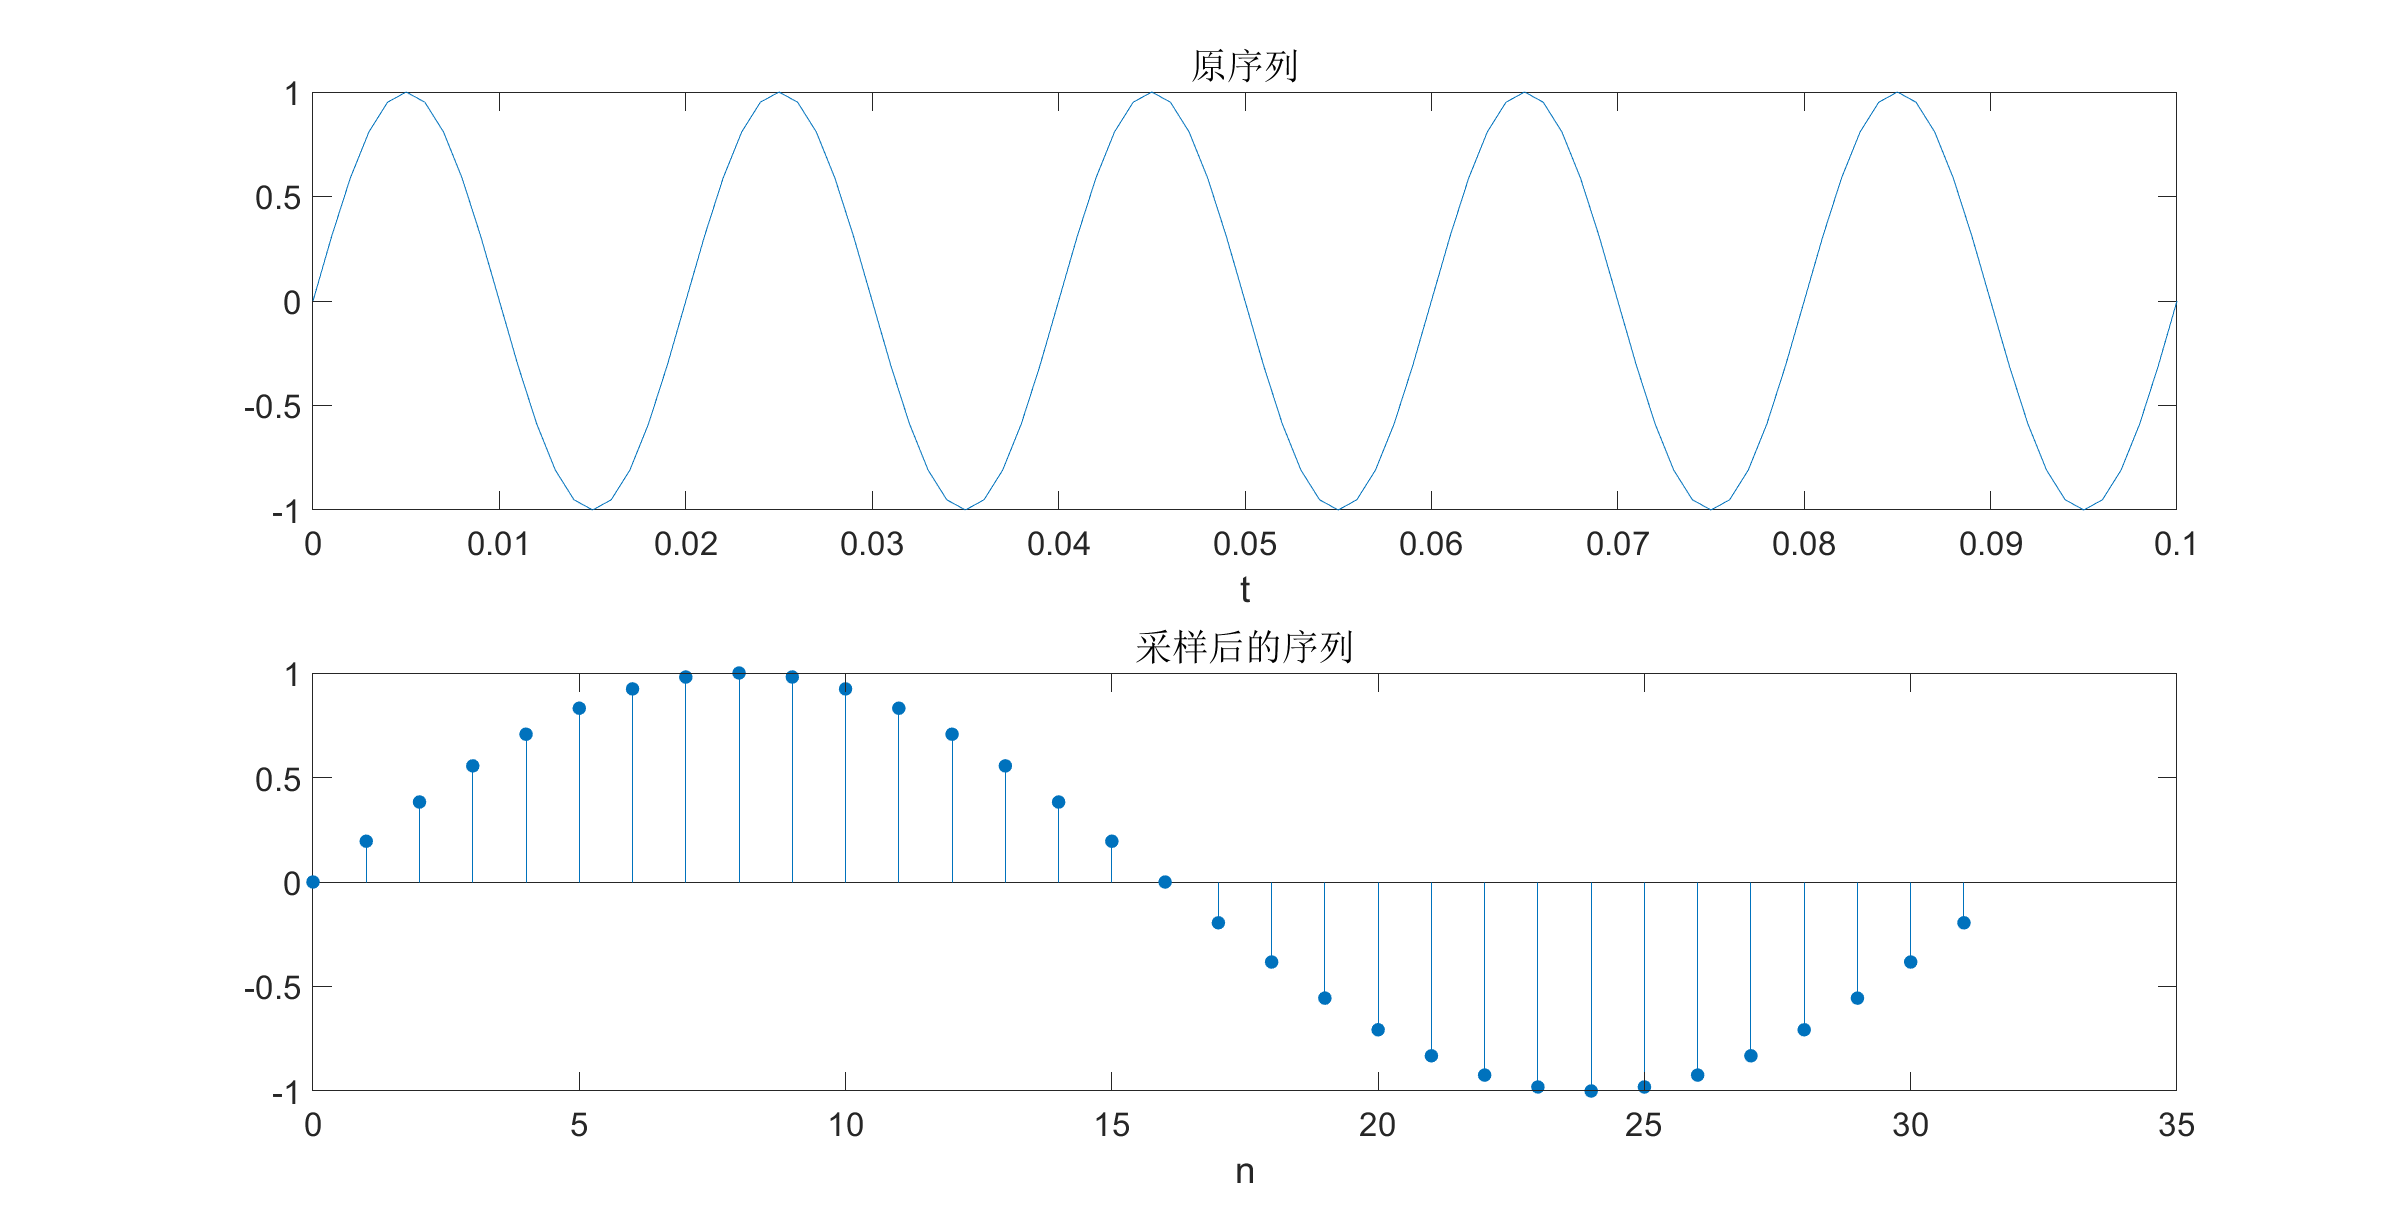
\includegraphics[width = \textwidth]{src/exp2_1_1.png}
                \end{figure}

                \begin{figure}[H]
                    \centering
                    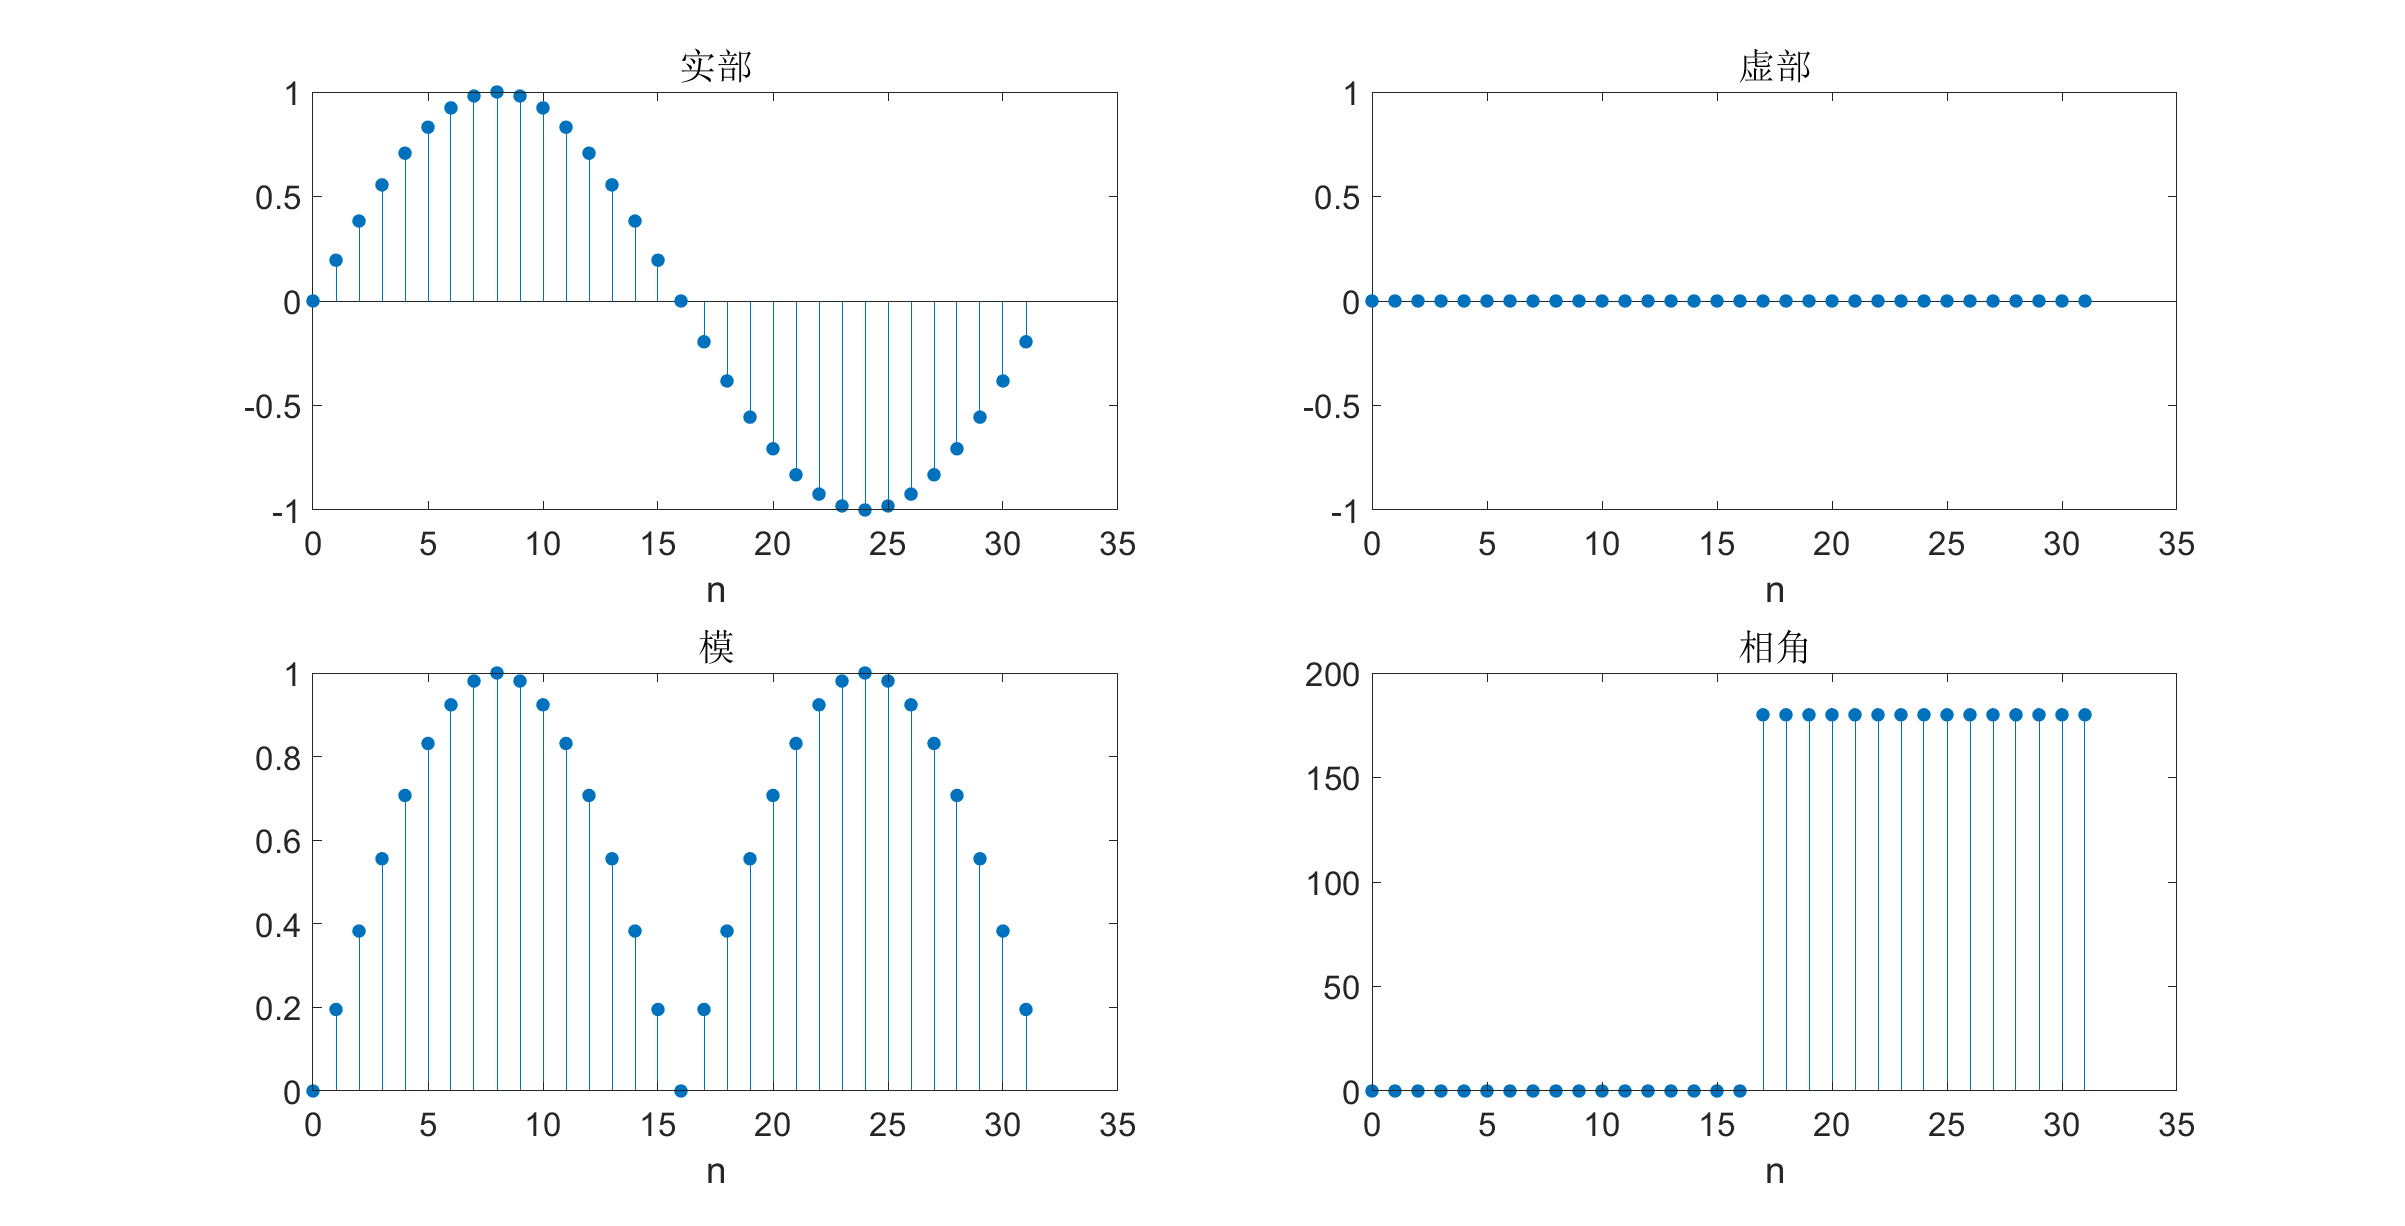
\includegraphics[width = \textwidth]{src/exp2_1_2.png}
                \end{figure}

                \begin{figure}[H]
                    \centering
                    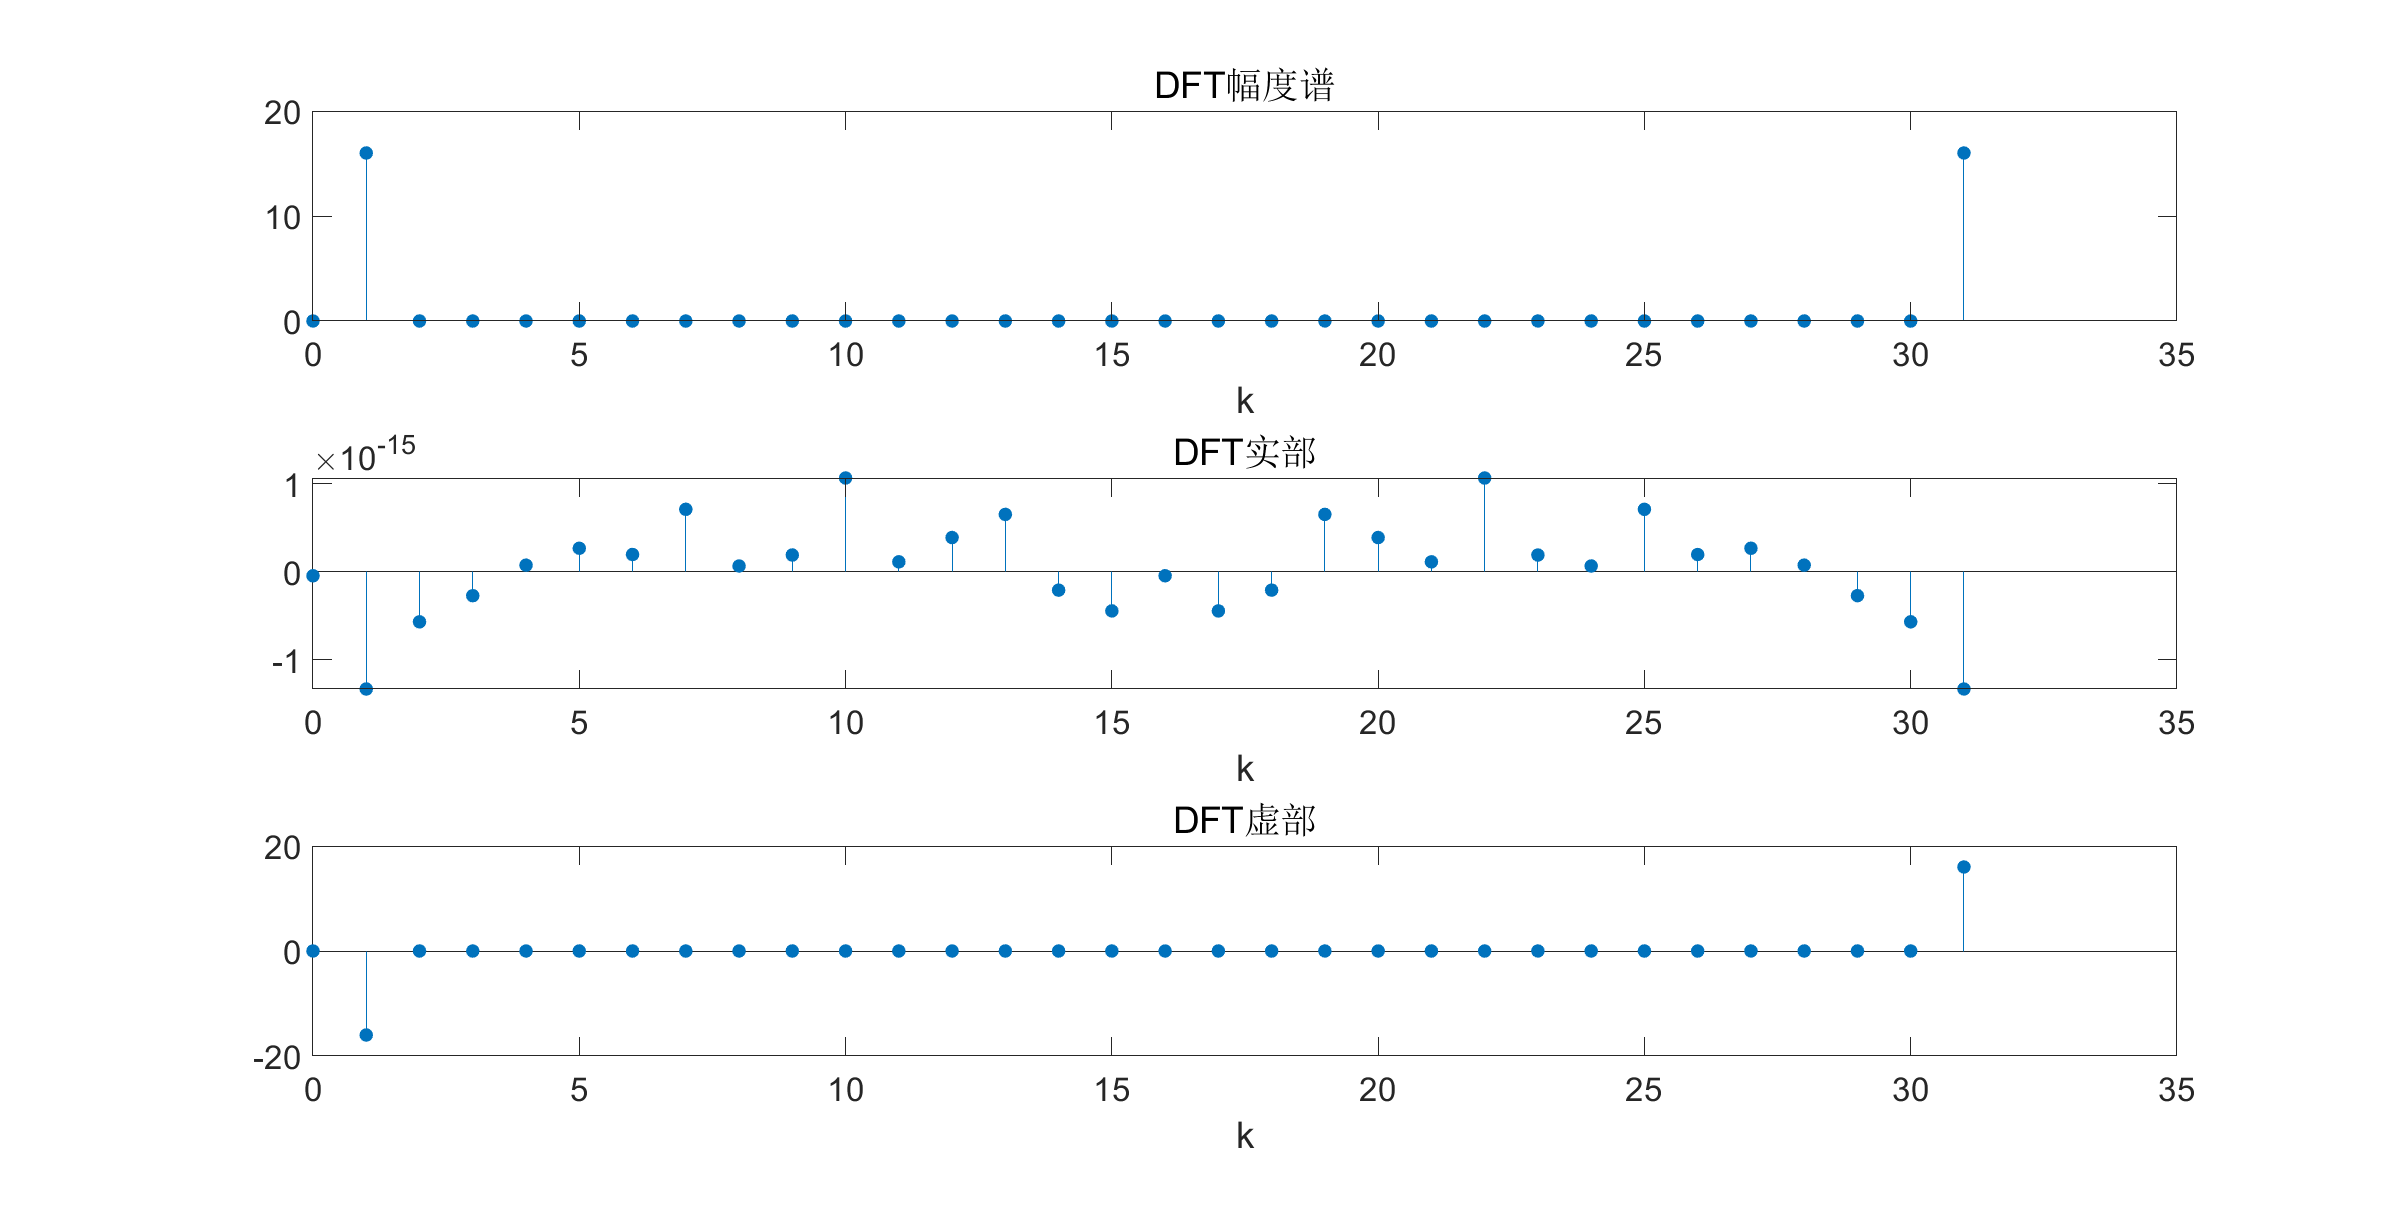
\includegraphics[width = \textwidth]{src/exp2_1_3.png}
                    \caption{第一组:f = 50Hz, T = 0.000625s, N = 32}
                \end{figure}

            \subsubsection{第二组参数}
                \begin{figure}[H]
                    \centering
                    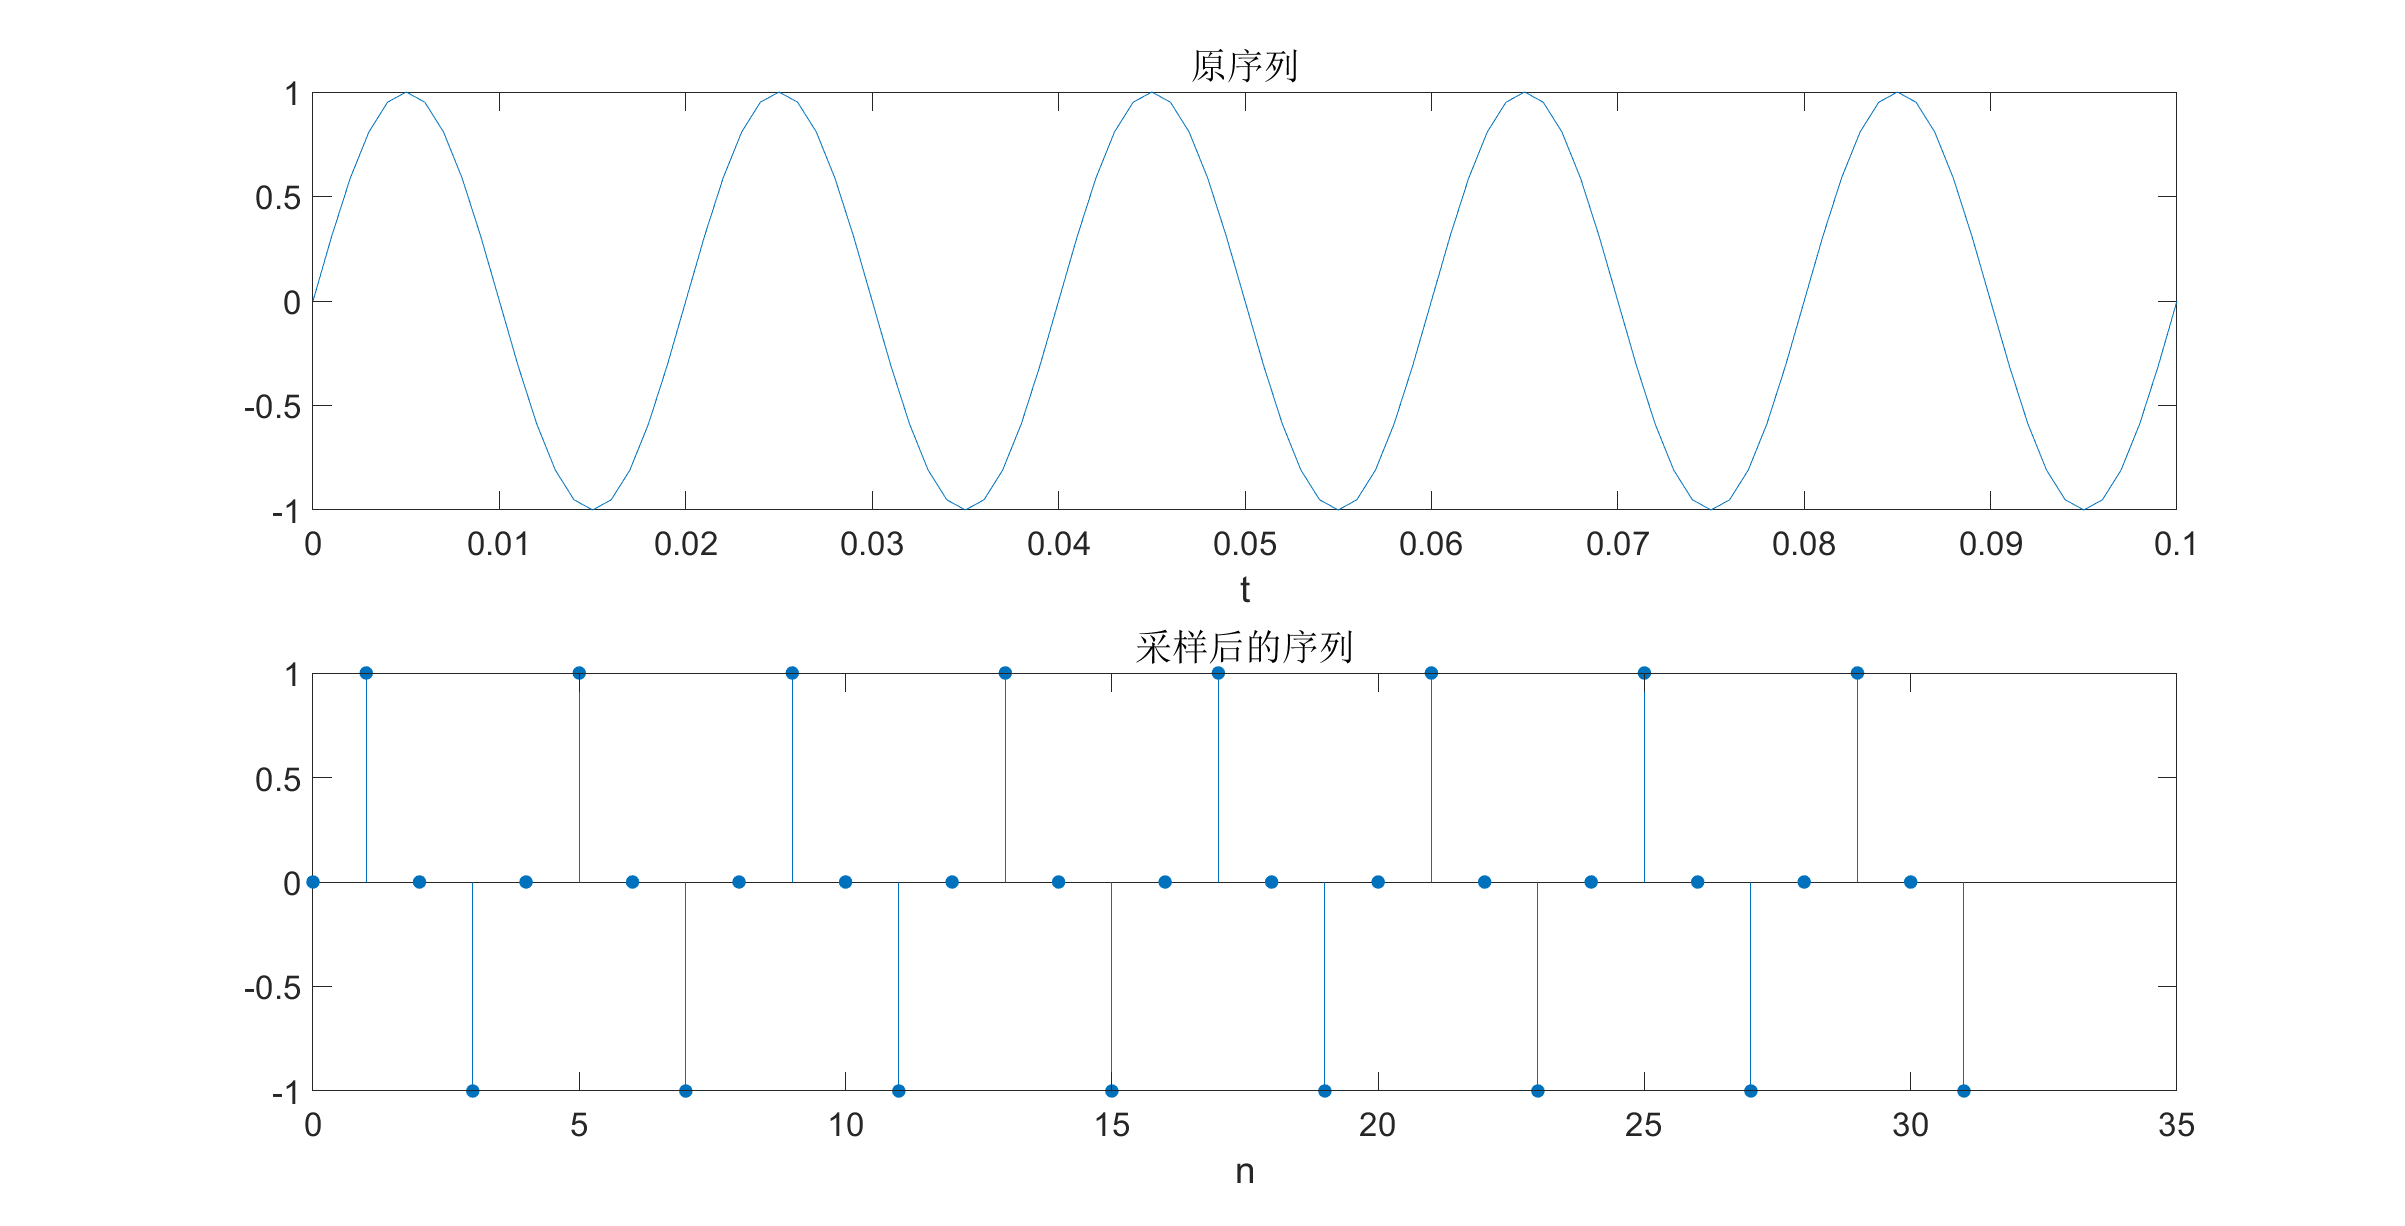
\includegraphics[width = \textwidth]{src/exp2_2_1.png}
                \end{figure}

                \begin{figure}[H]
                    \centering
                    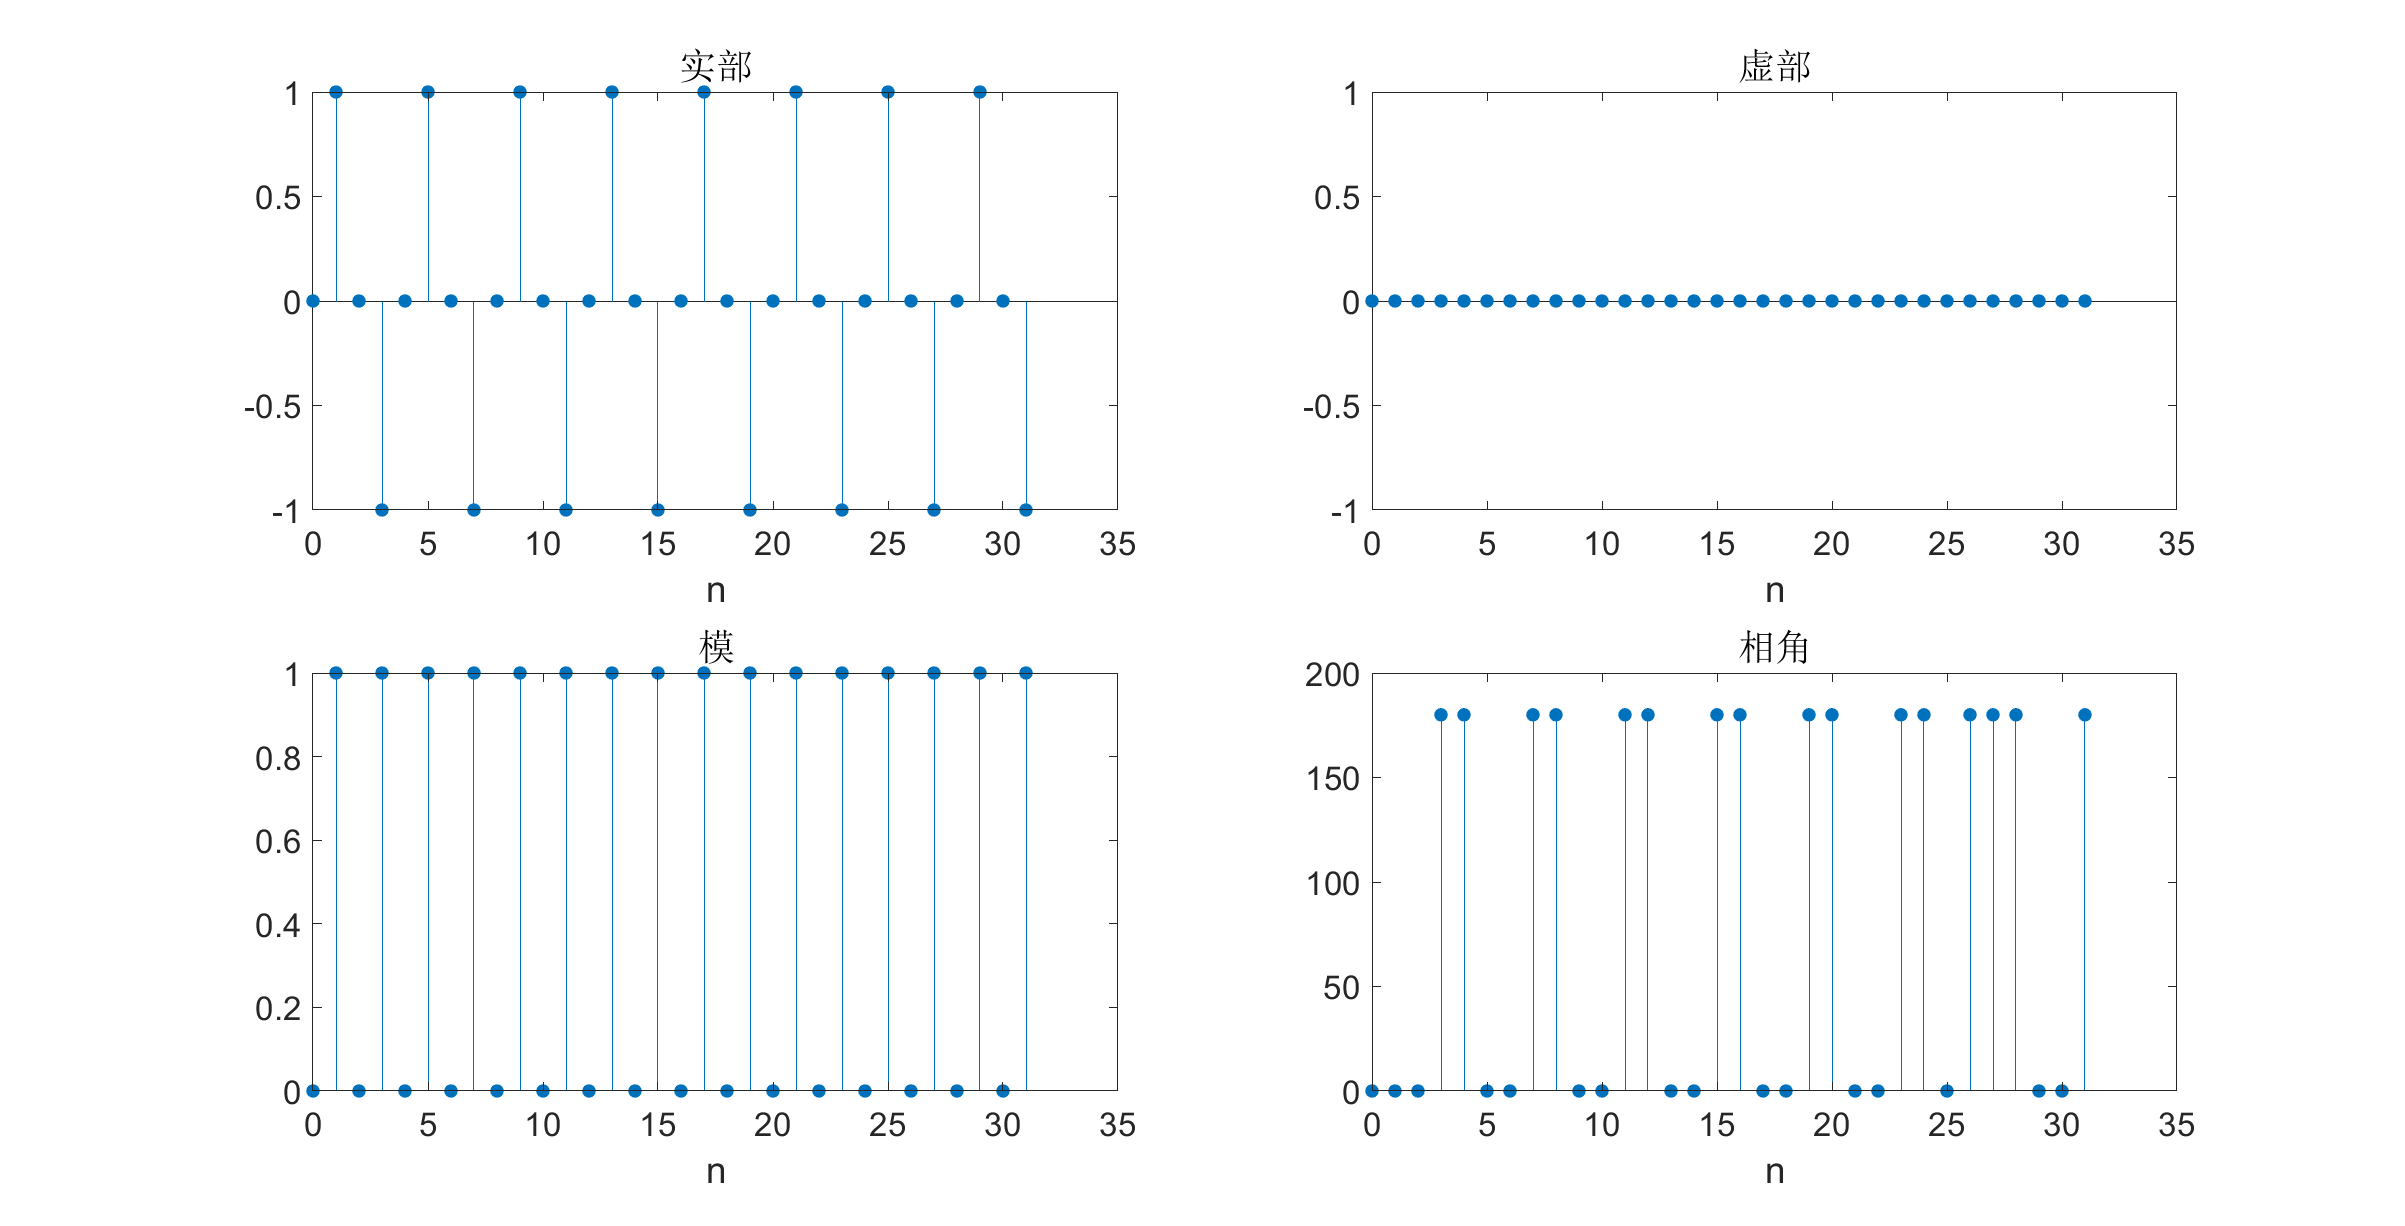
\includegraphics[width = \textwidth]{src/exp2_2_2.png}
                \end{figure}

                \begin{figure}[H]
                    \centering
                    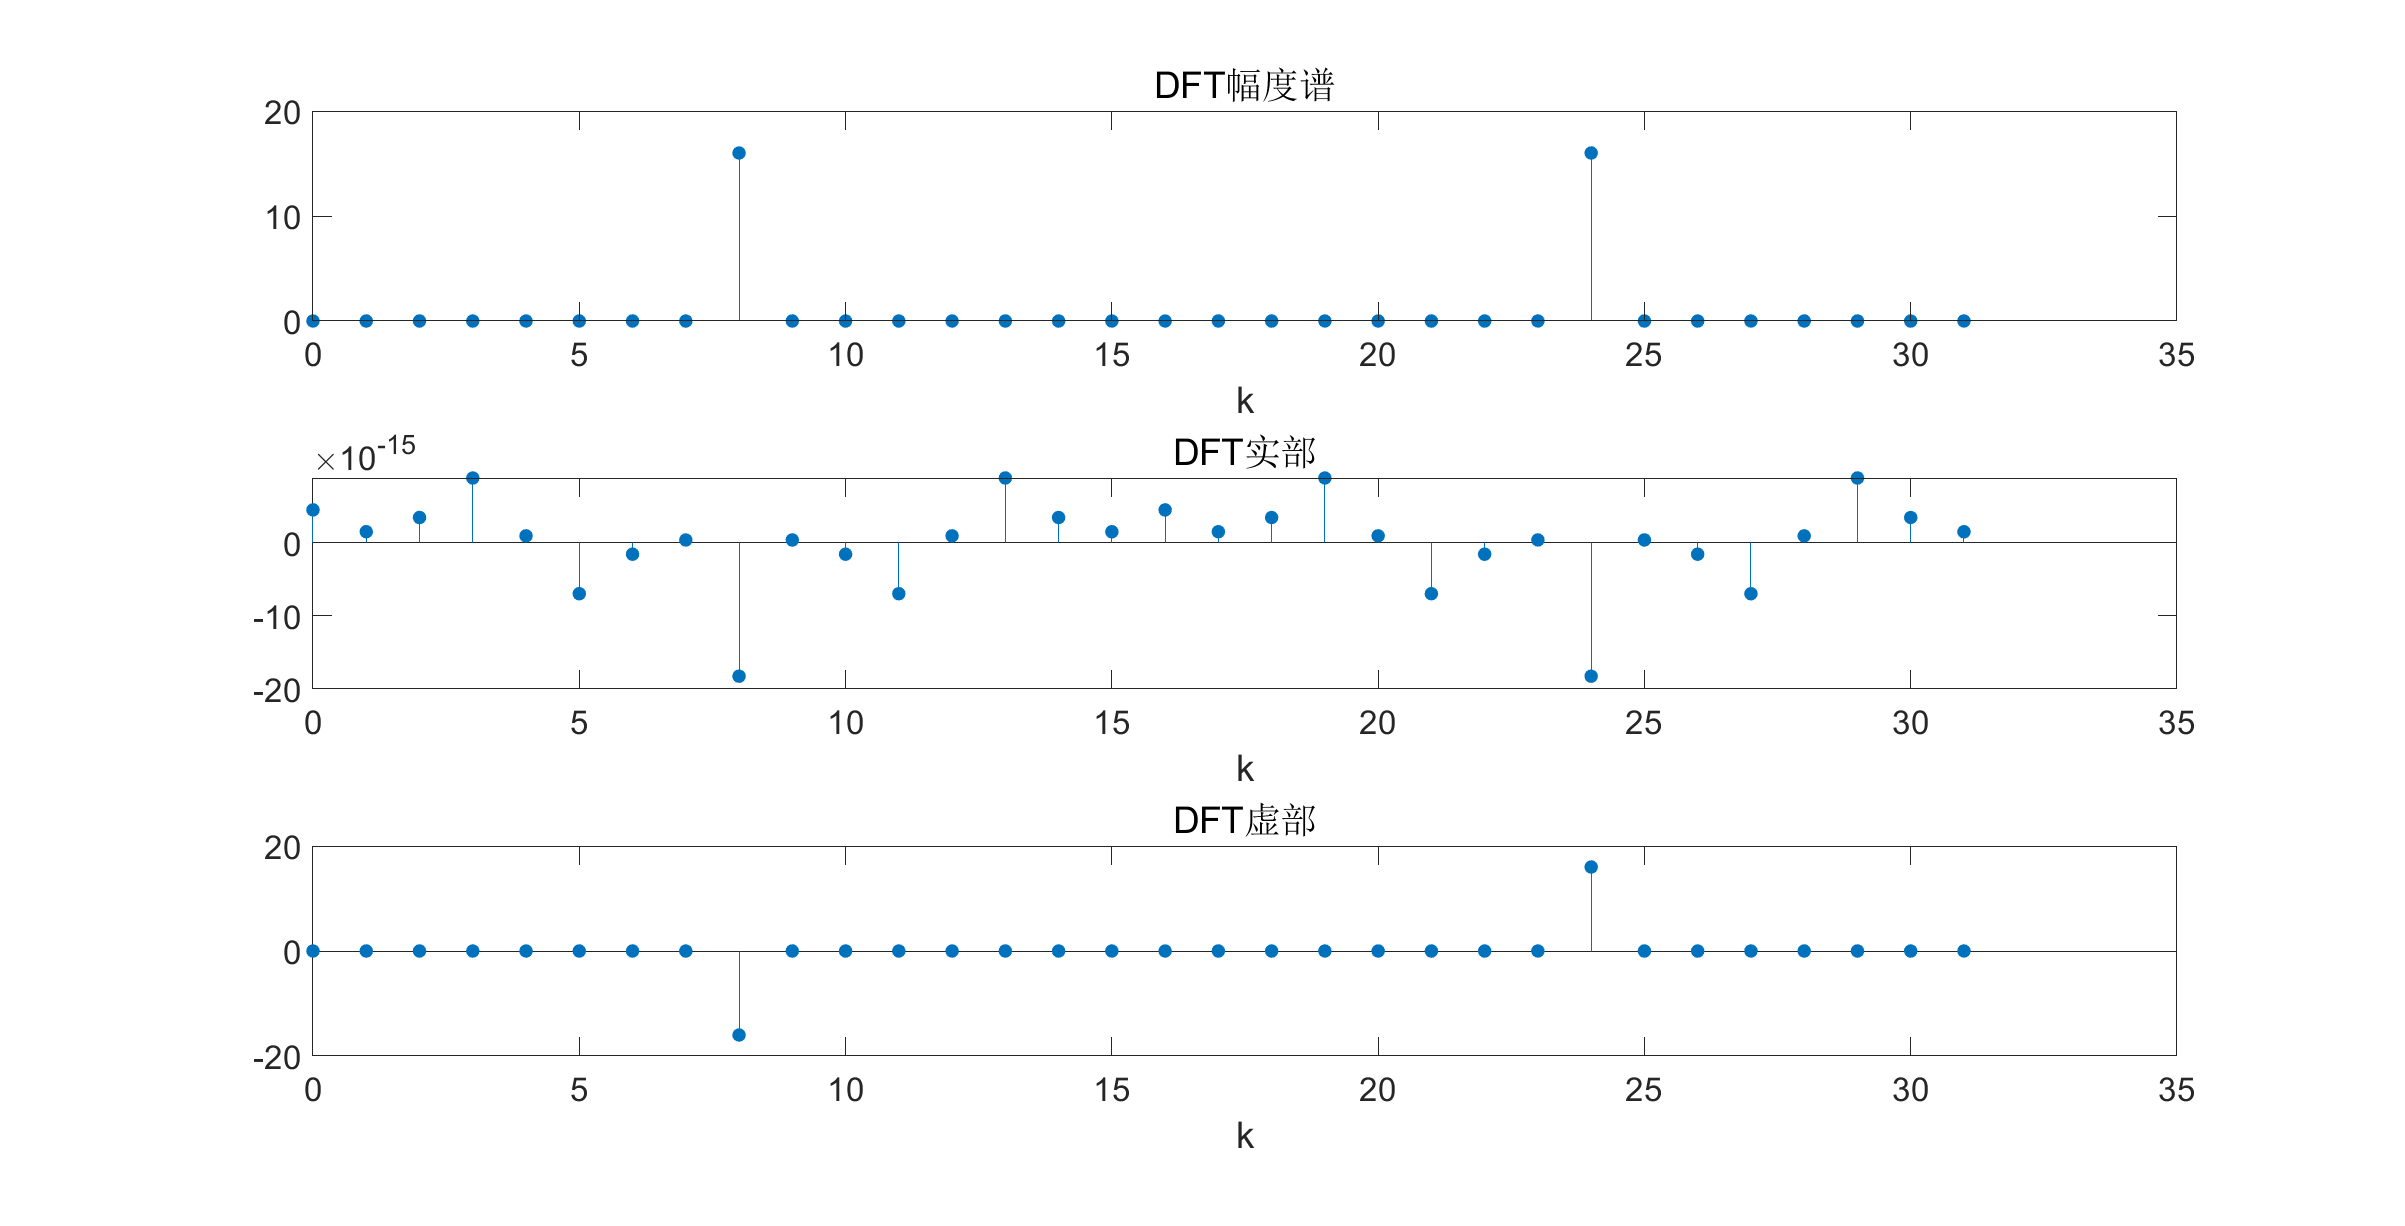
\includegraphics[width = \textwidth]{src/exp2_2_3.png}
                    \caption{第二组:f = 50Hz, T = 0.005s, N = 32}
                \end{figure}

            \subsubsection{第三组参数}
                \begin{figure}[H]
                    \centering
                    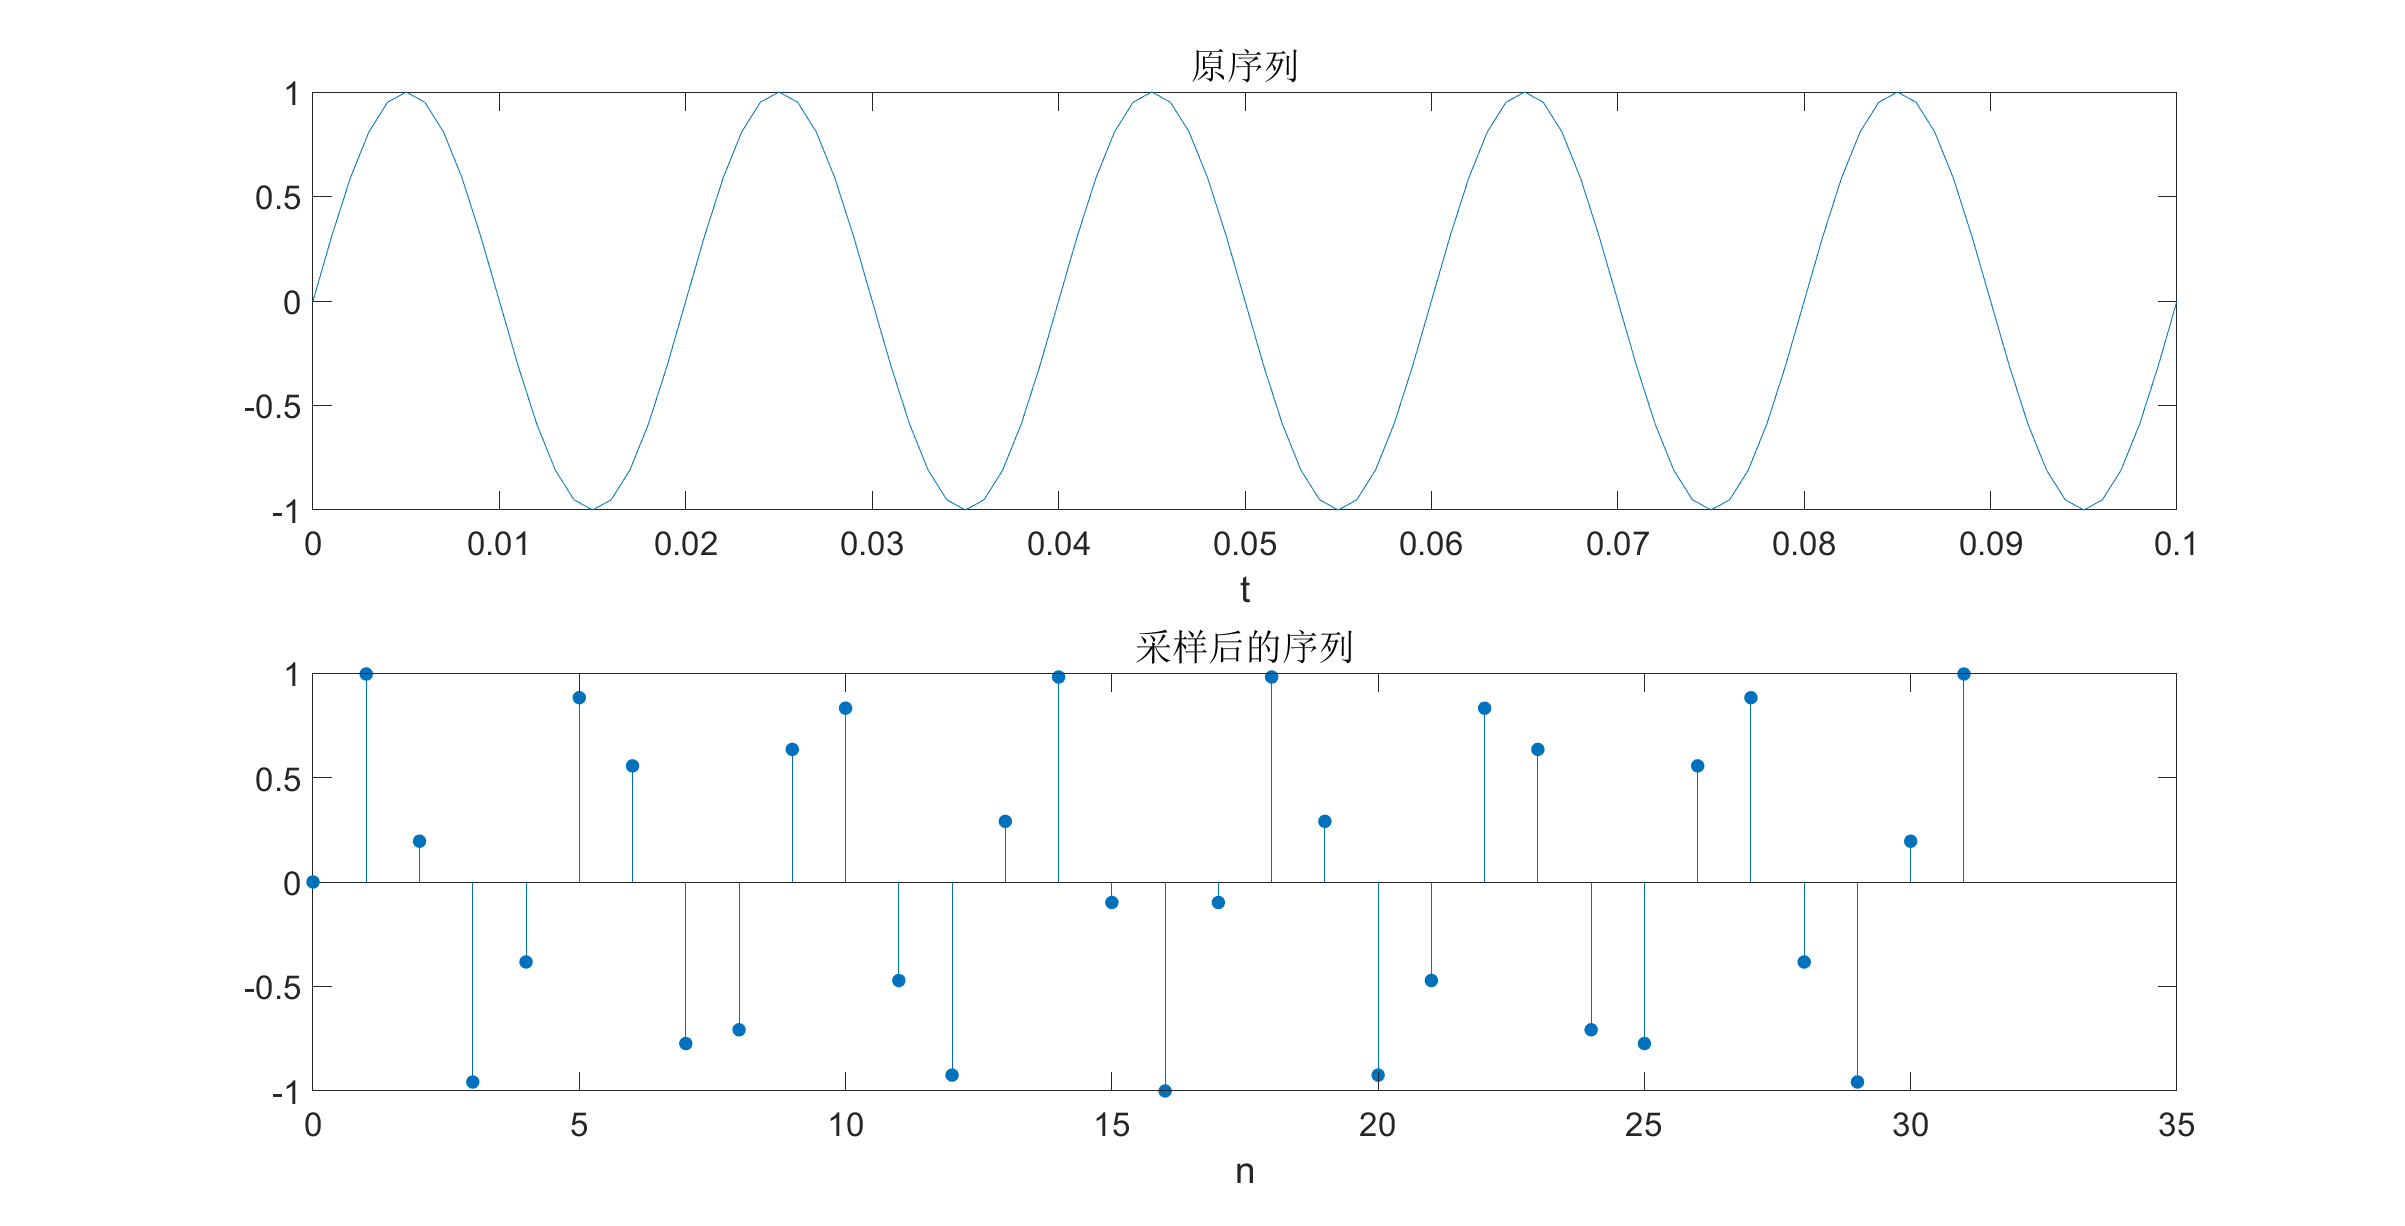
\includegraphics[width = \textwidth]{src/exp2_3_1.png}
                \end{figure}

                \begin{figure}[H]
                    \centering
                    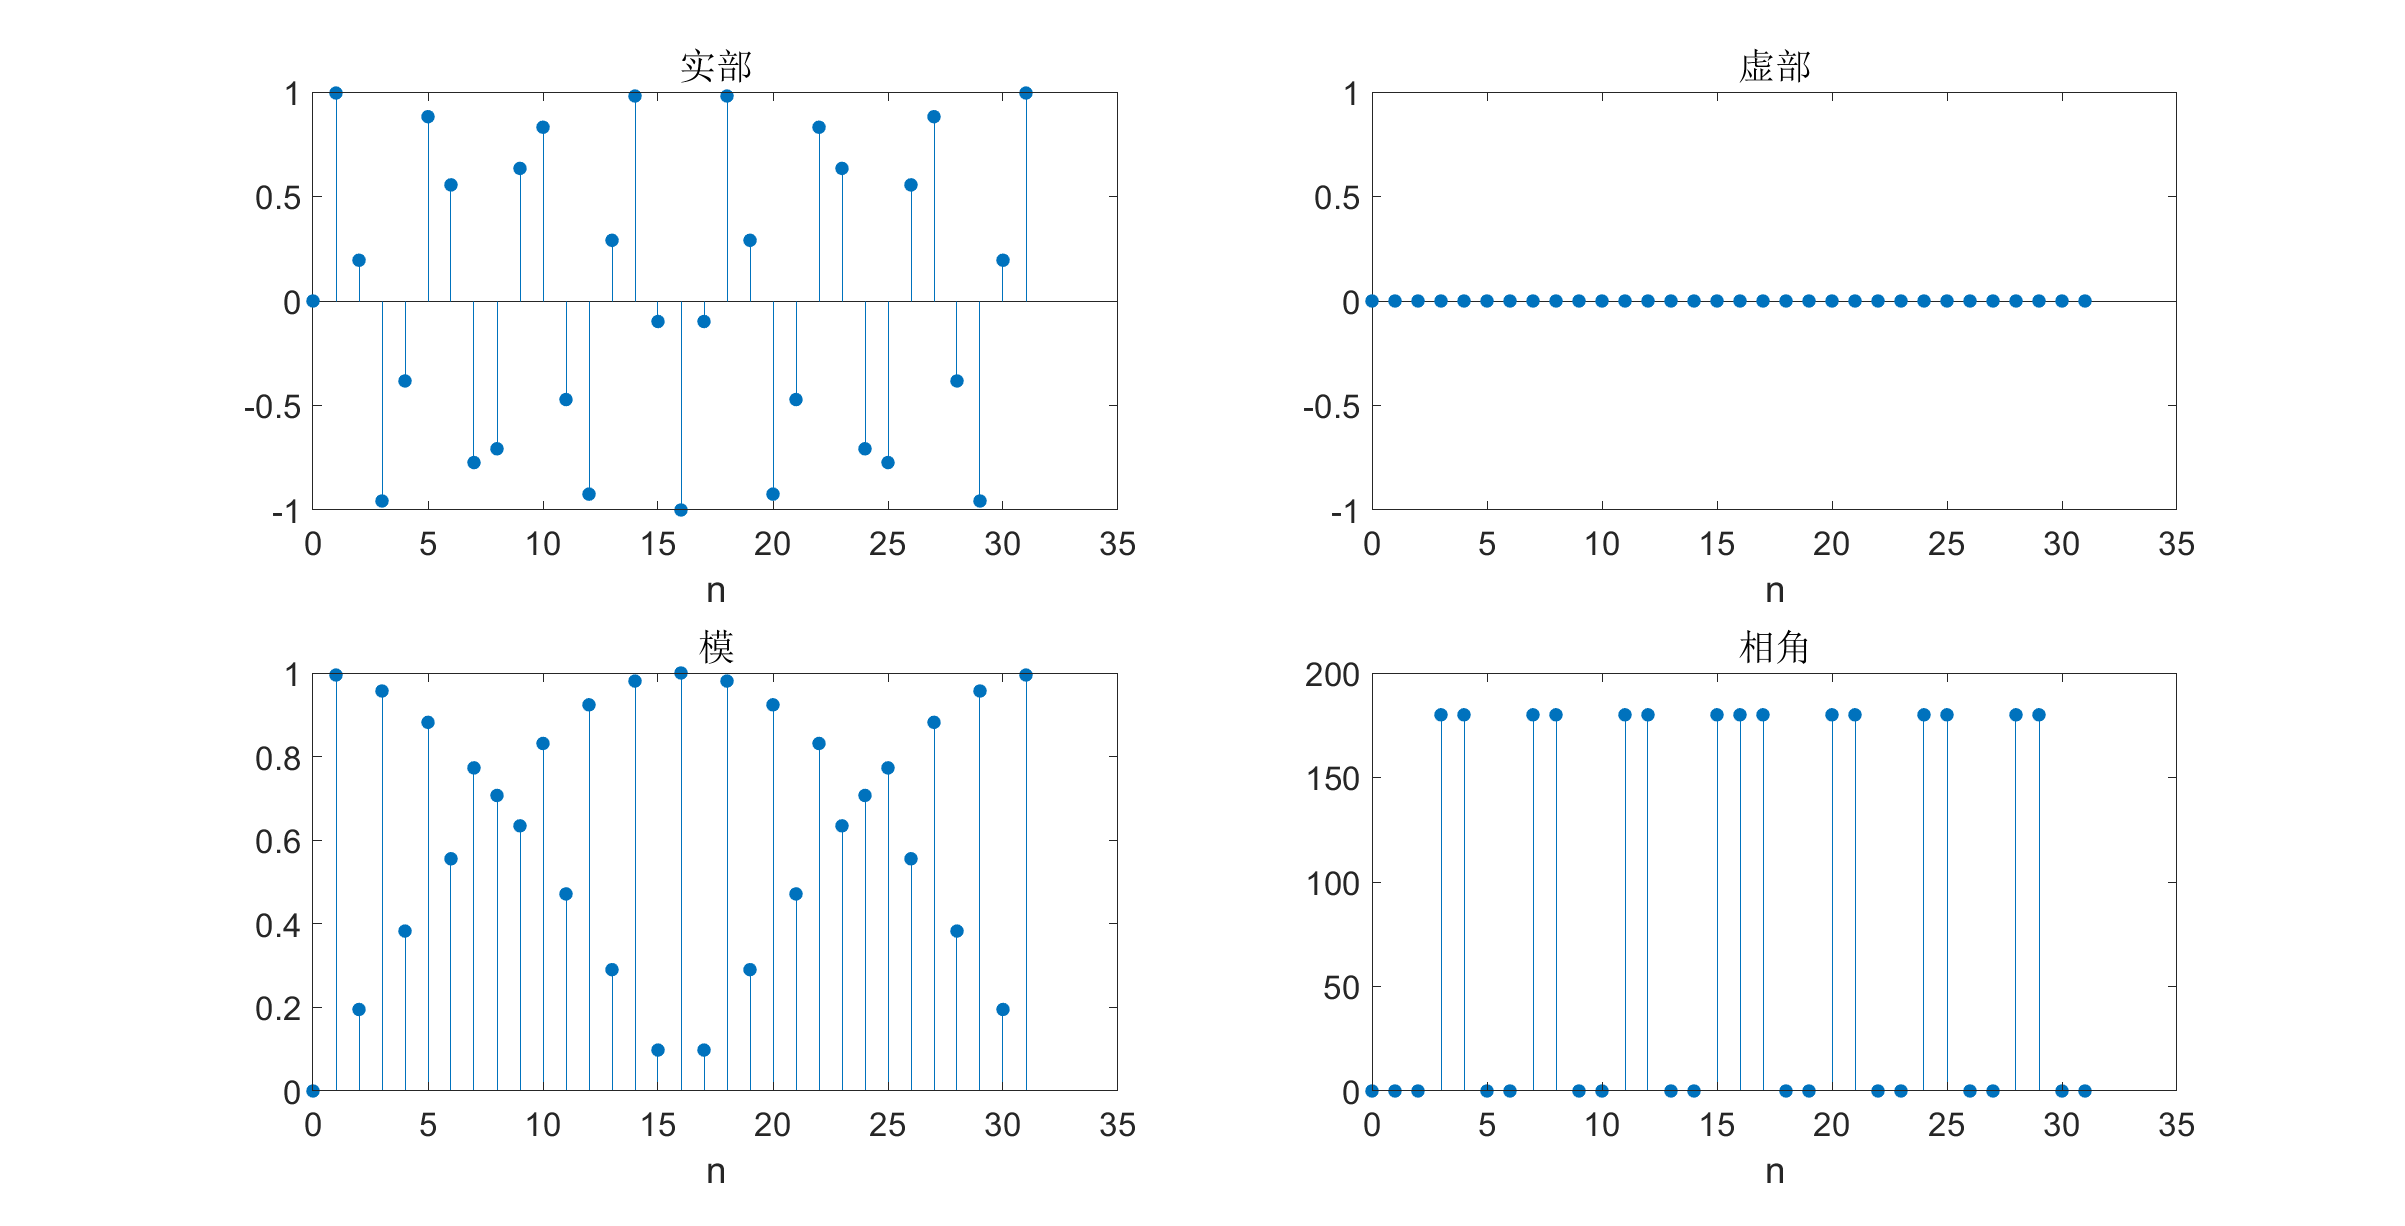
\includegraphics[width = \textwidth]{src/exp2_3_2.png}
                \end{figure}

                \begin{figure}[H]
                    \centering
                    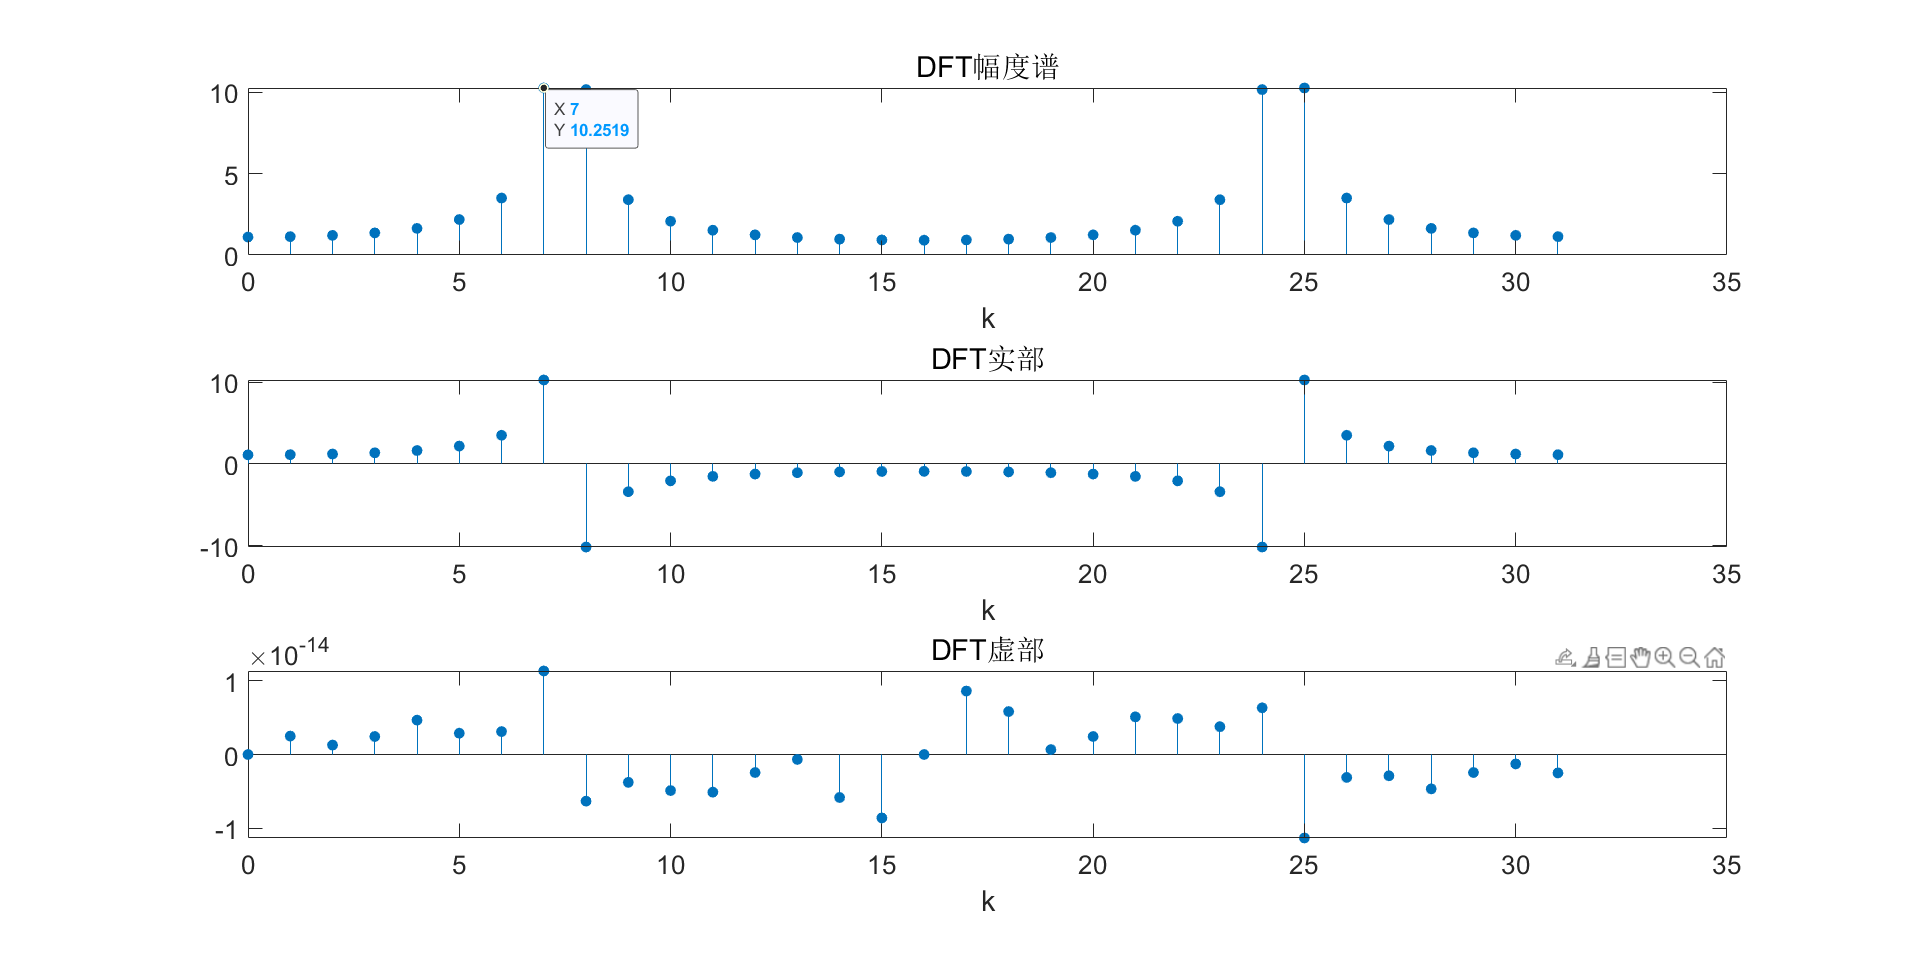
\includegraphics[width = \textwidth]{src/exp2_3_3.png}
                    \caption{第三组:f = 50Hz, T = 0.0046875s, N = 32}
                \end{figure}
            可以看见,此组出现了频谱泄露的现象。
            \subsubsection{第四组参数}
                \begin{figure}[H]
                    \centering
                    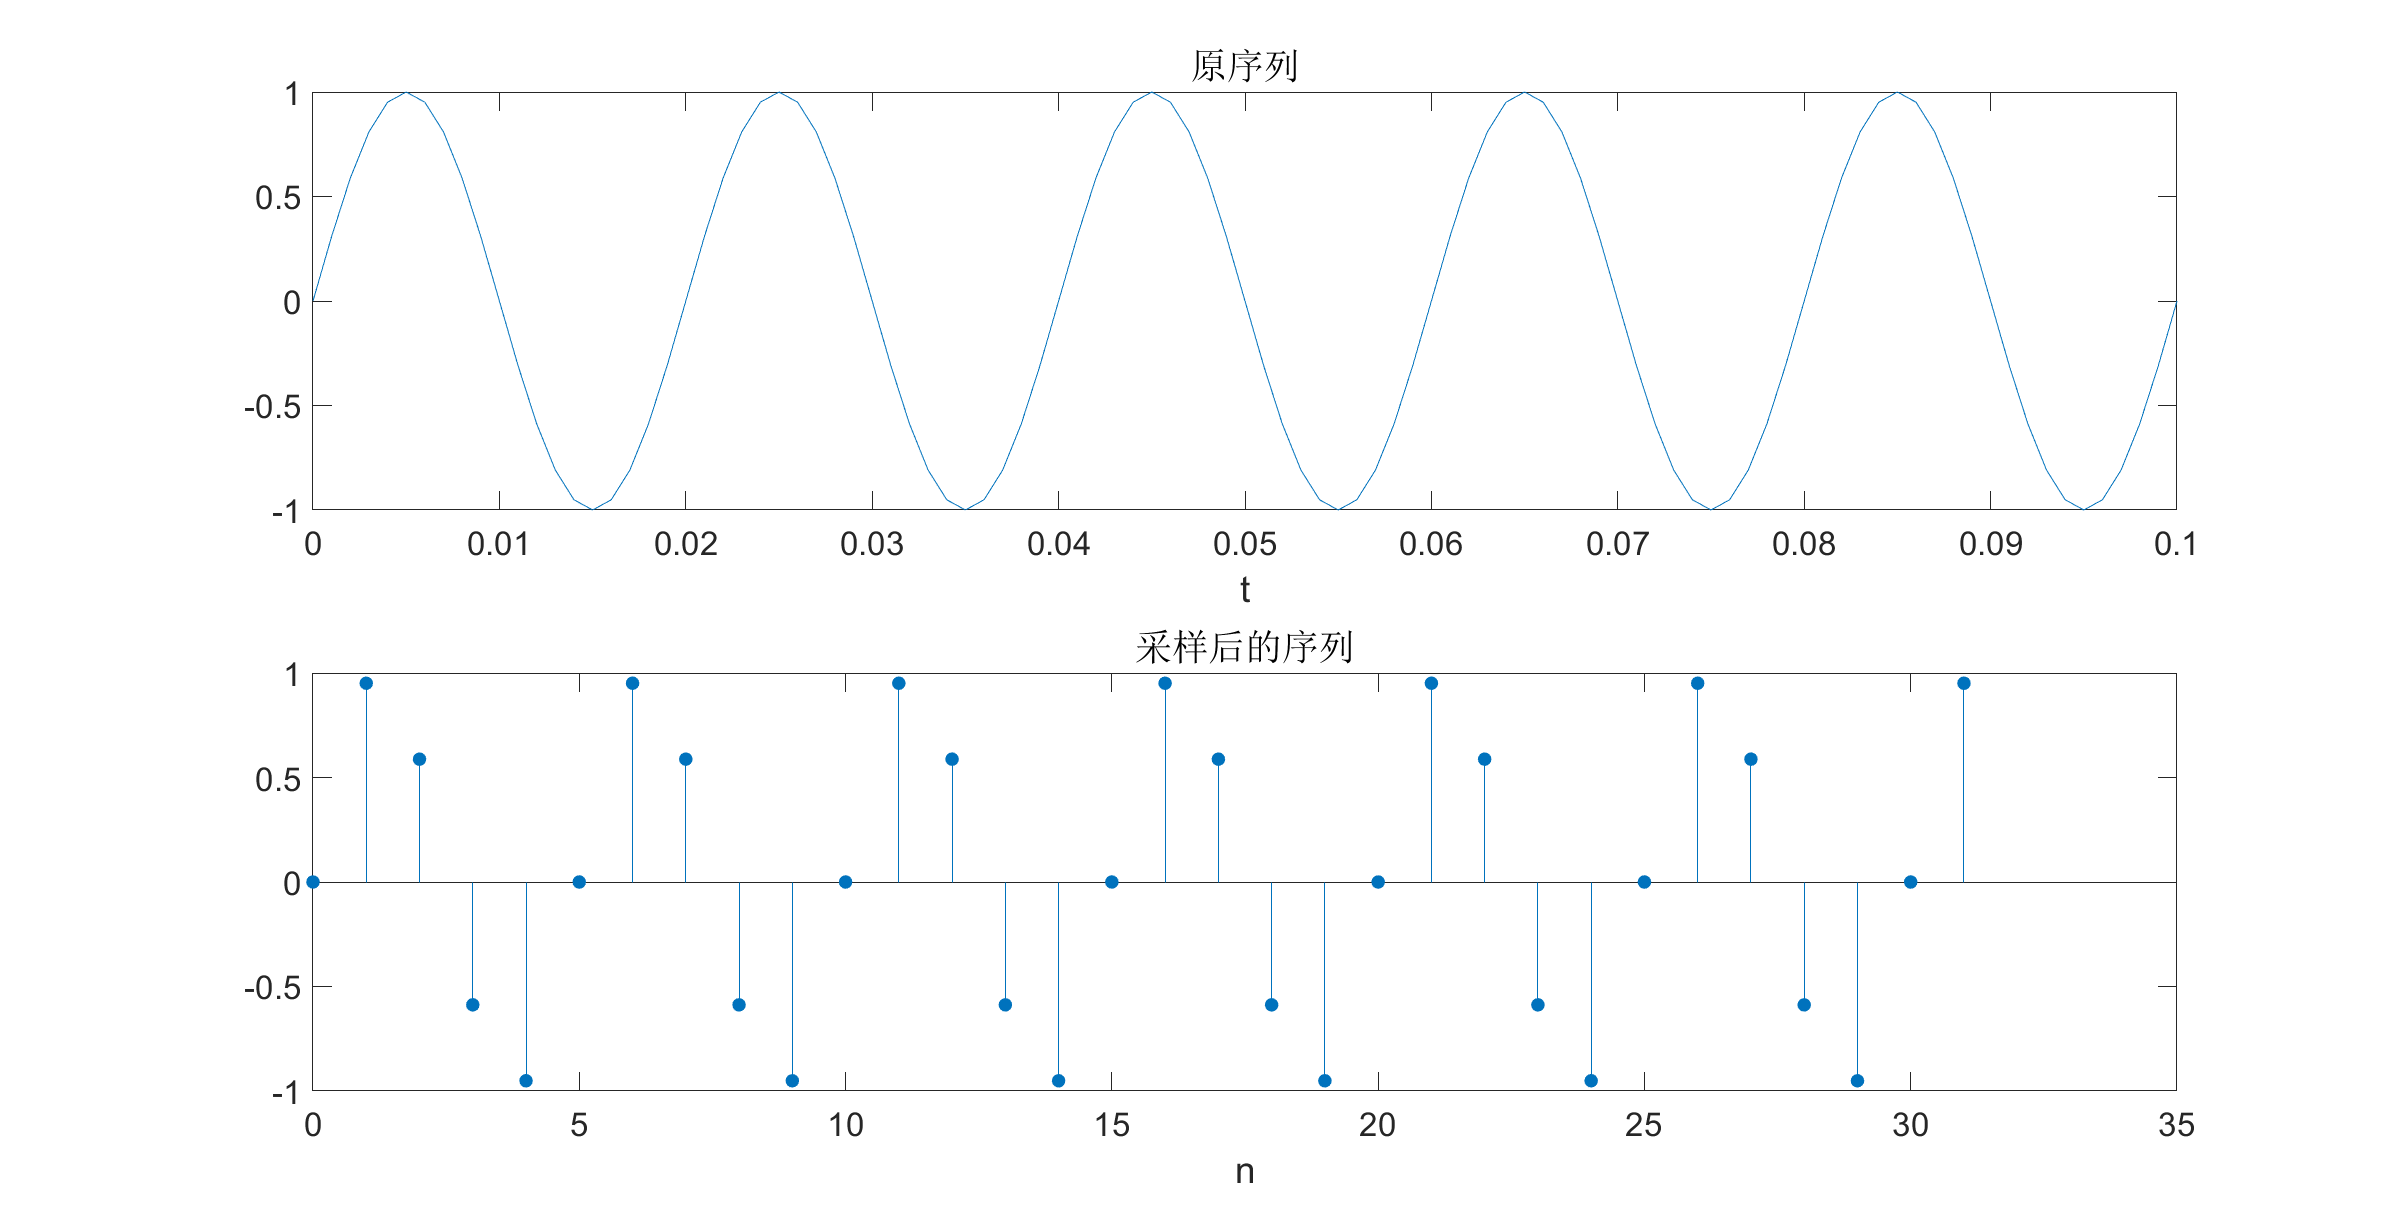
\includegraphics[width = \textwidth]{src/exp2_4_1.png}
                \end{figure}

                \begin{figure}[H]
                    \centering
                    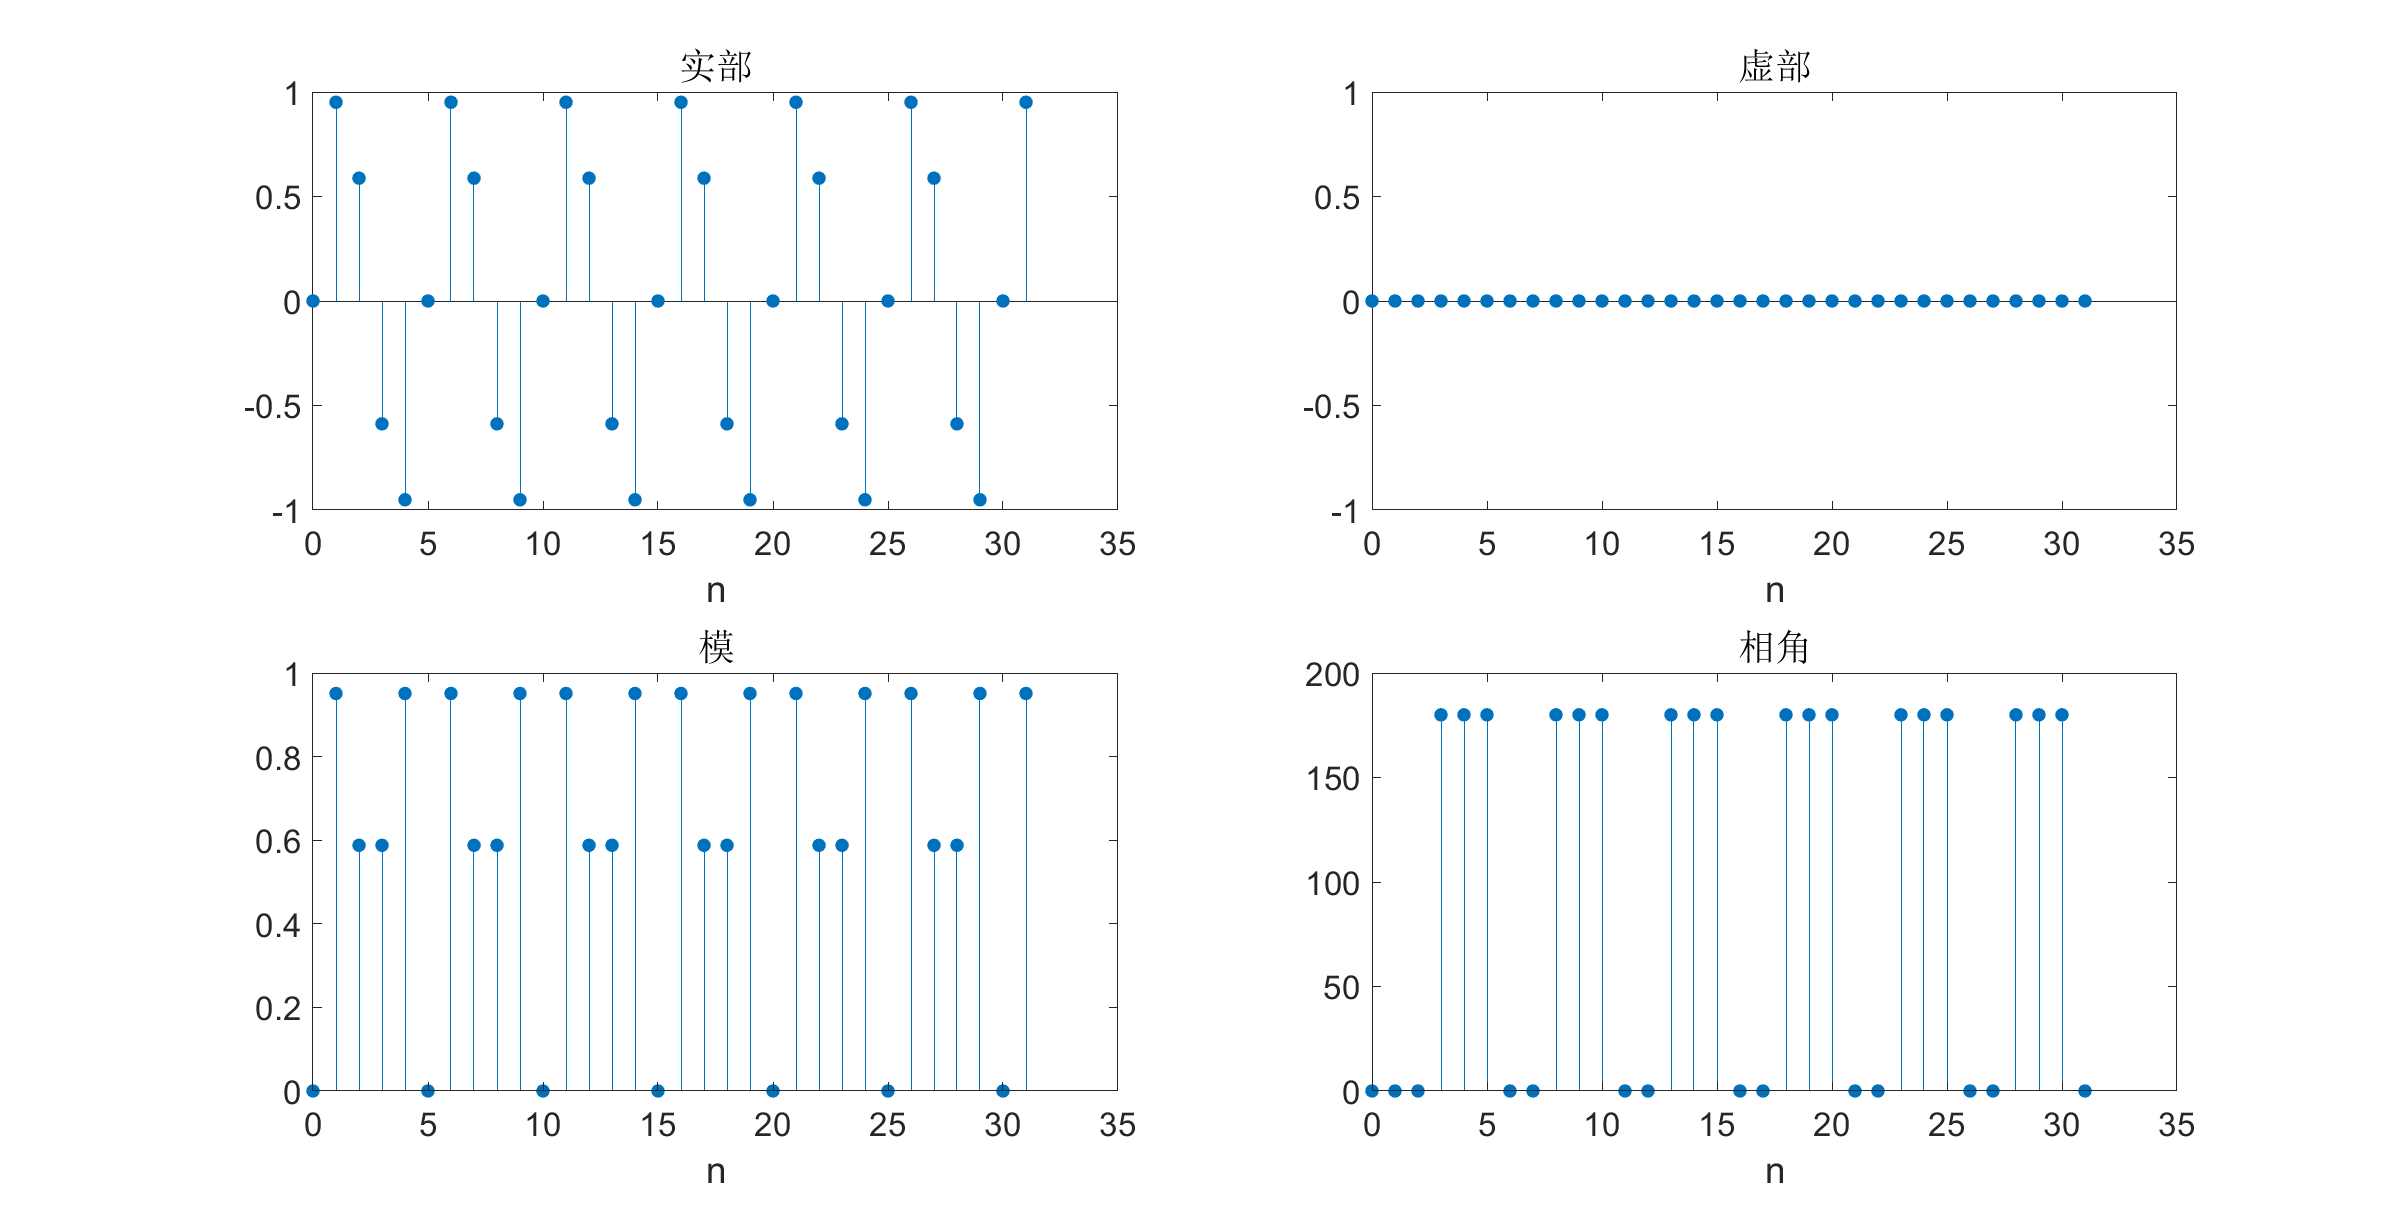
\includegraphics[width = \textwidth]{src/exp2_4_2.png}
                \end{figure}

                \begin{figure}[H]
                    \centering
                    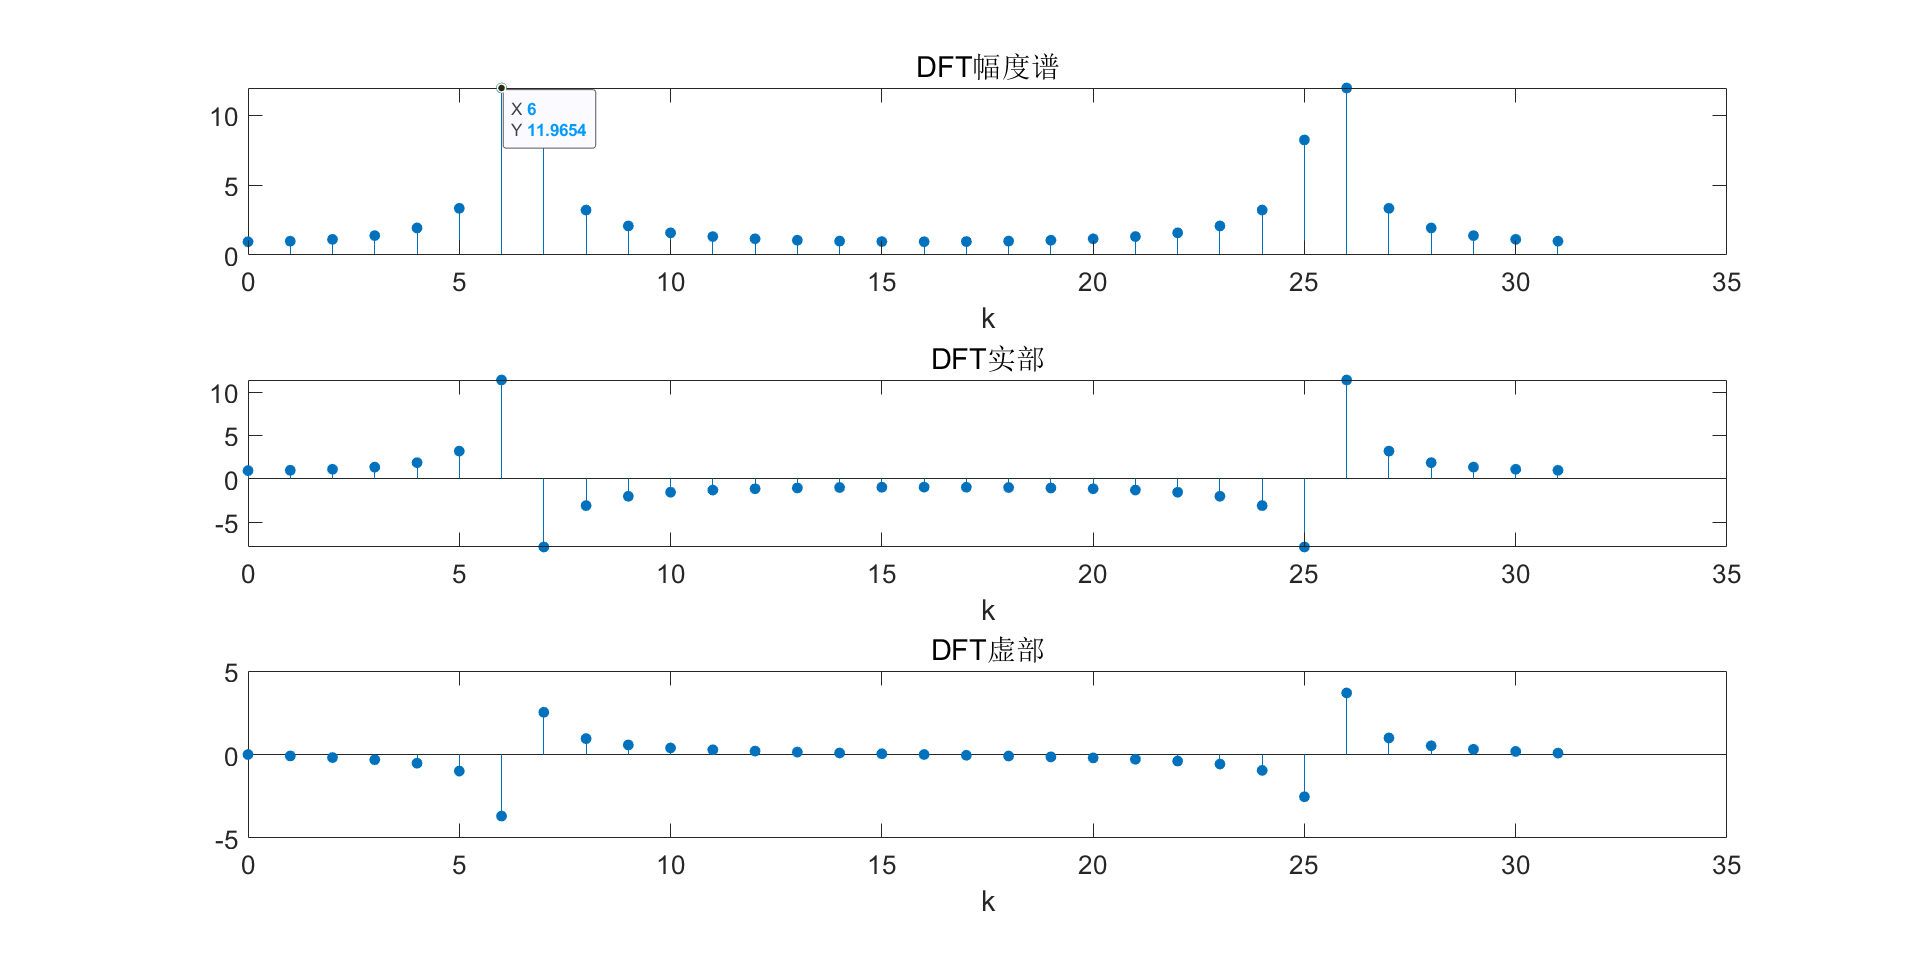
\includegraphics[width = \textwidth]{src/exp2_4_3.png}
                    \caption{第四组:f = 50Hz, T = 0.004s, N = 32}
                \end{figure}
            可以看见,此组出现了频谱泄露的现象。
            \subsubsection{第五组参数}
                \begin{figure}[H]
                    \centering
                    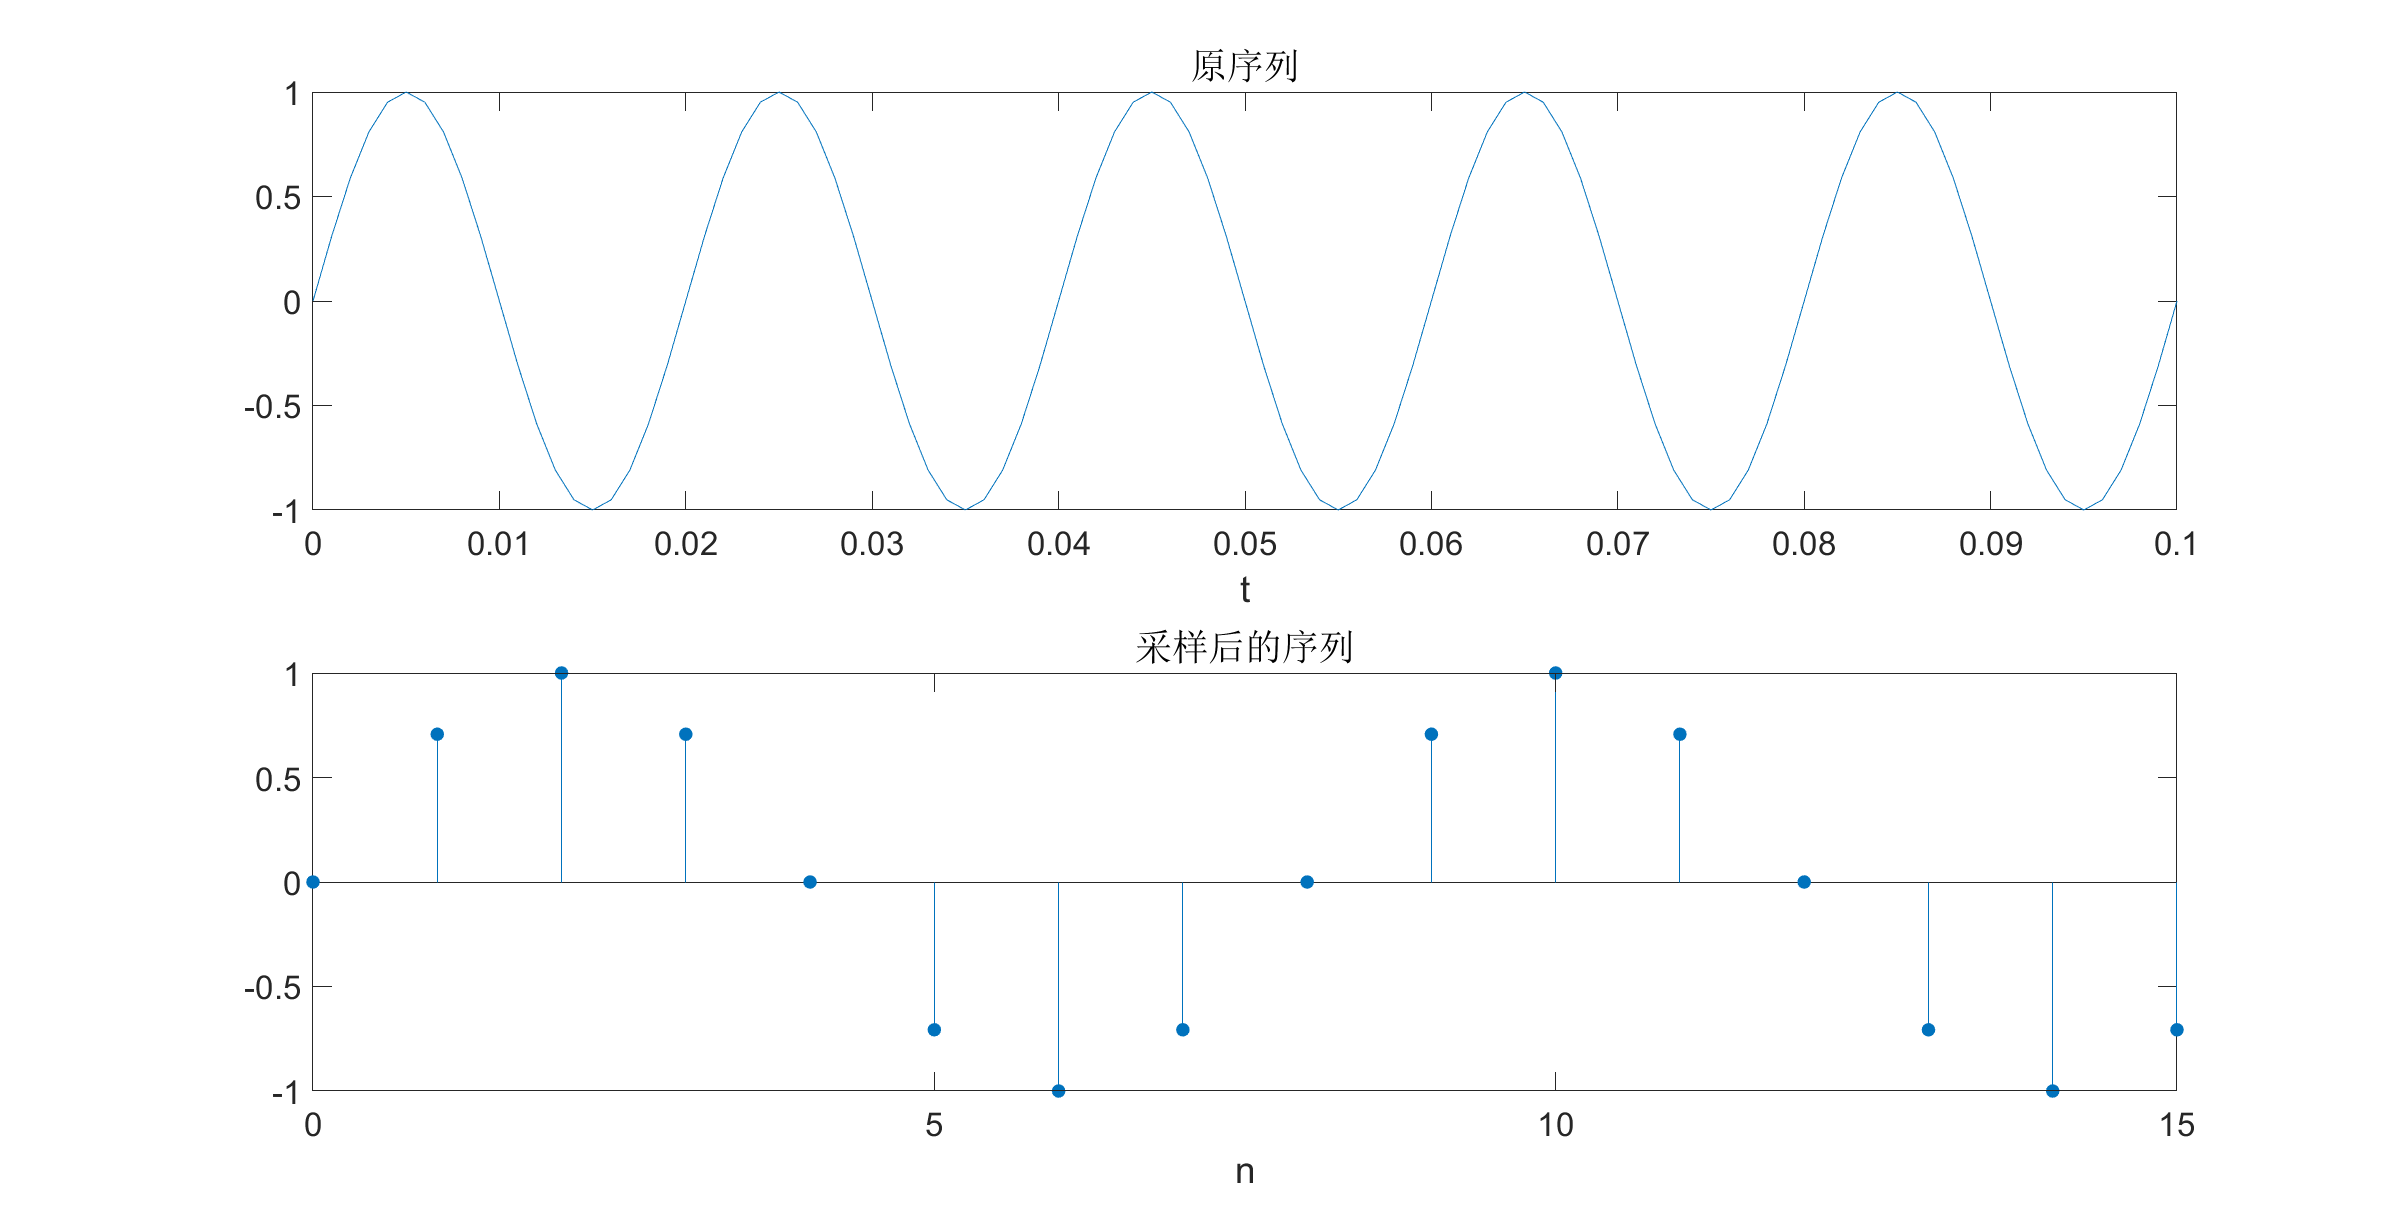
\includegraphics[width = \textwidth]{src/exp2_5_1.png}
                \end{figure}

                \begin{figure}[H]
                    \centering
                    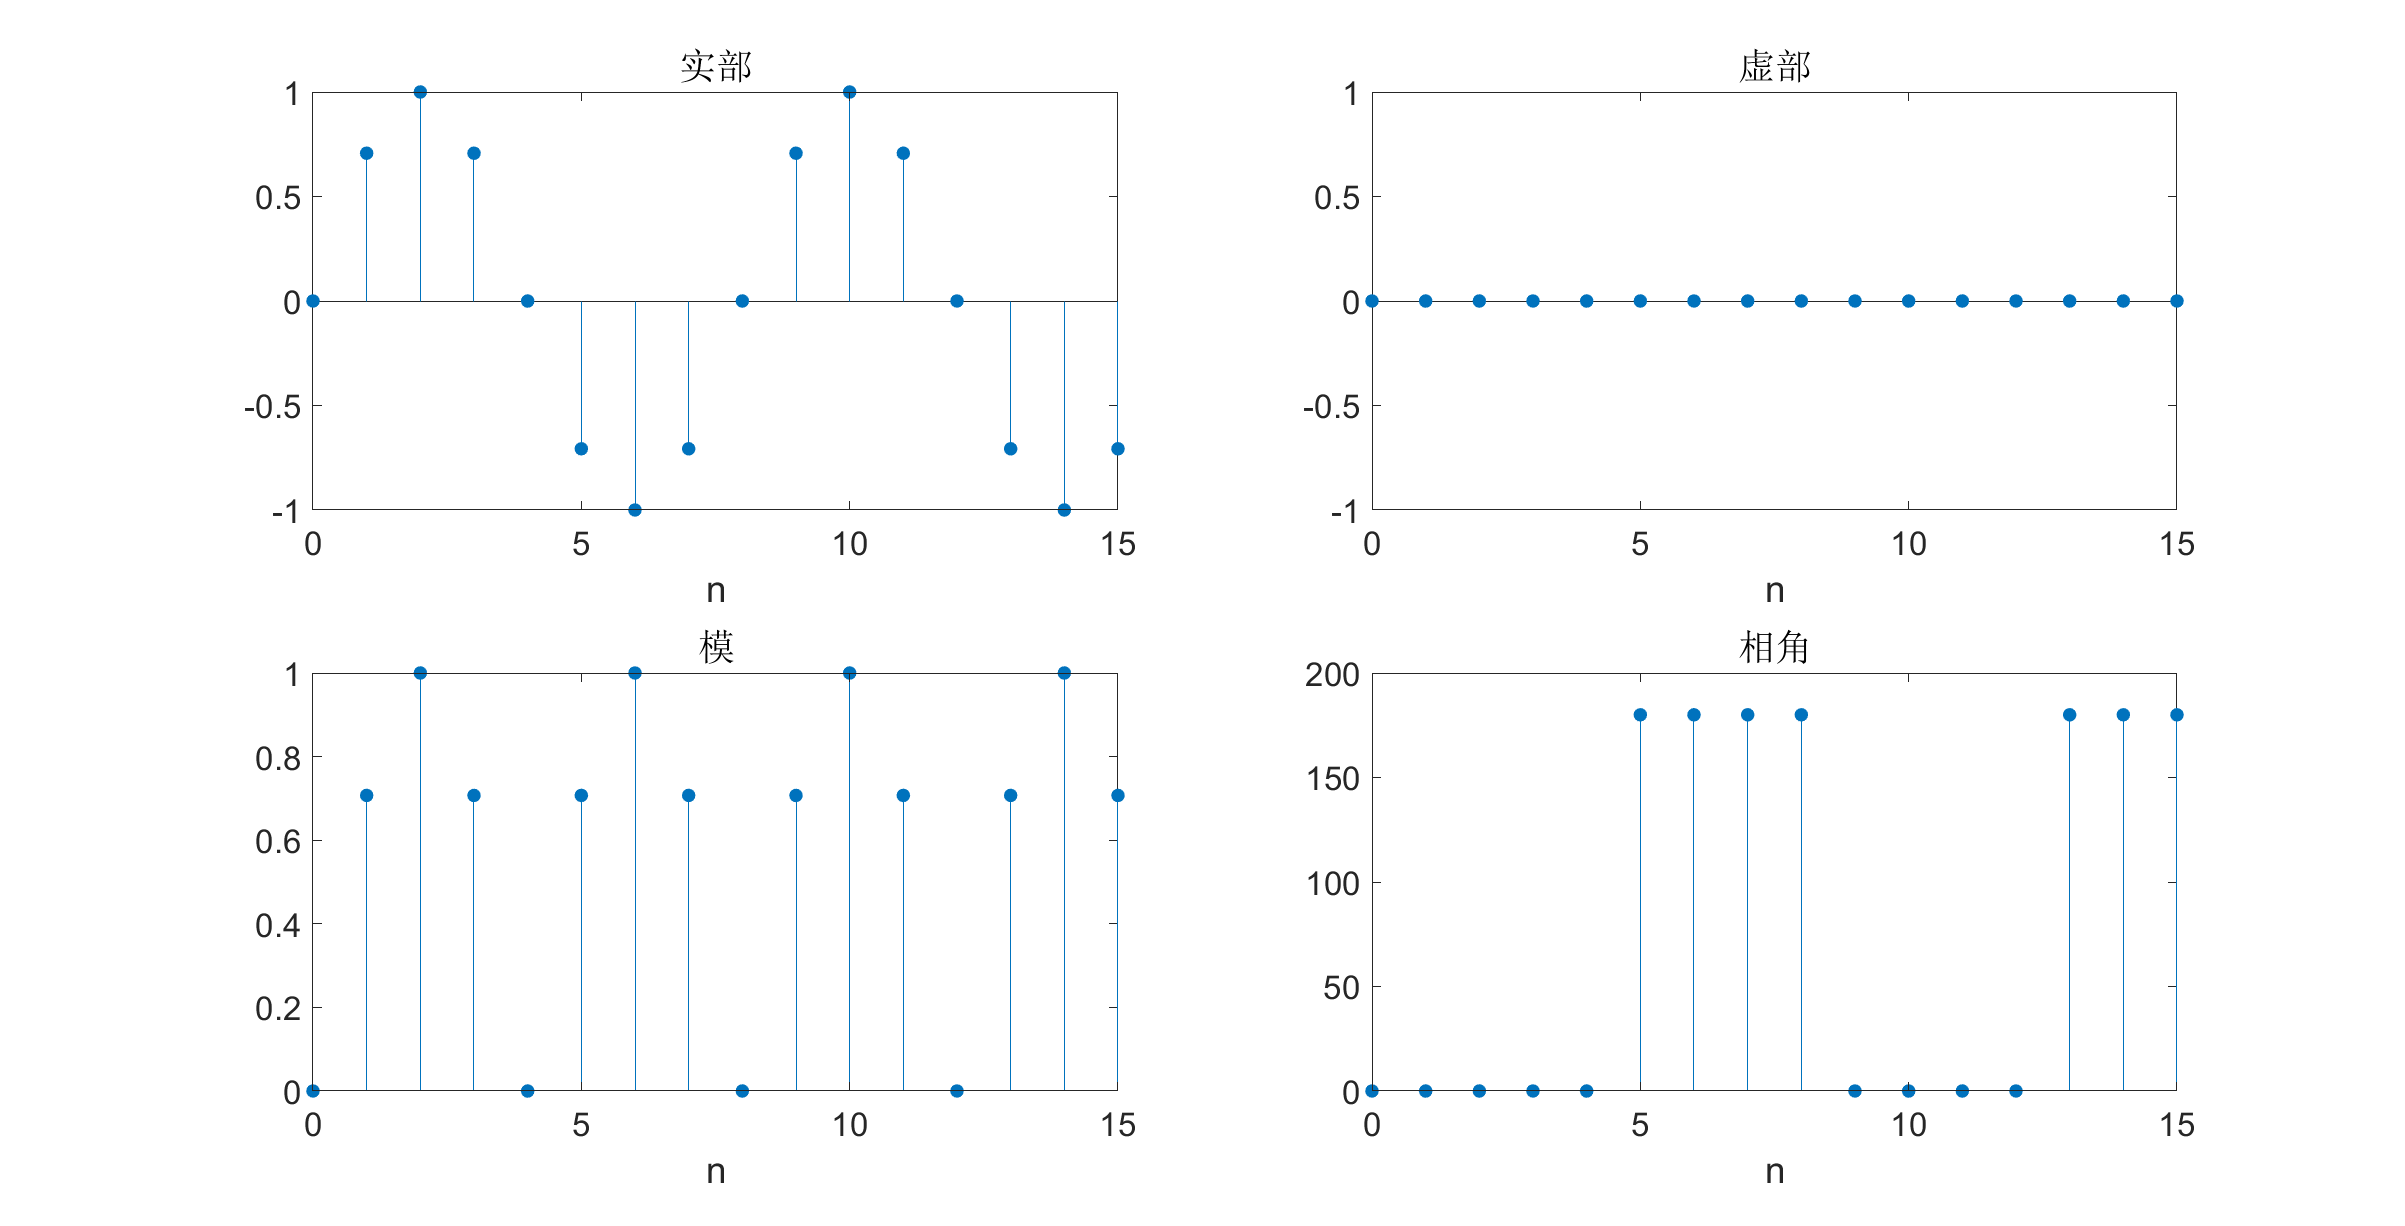
\includegraphics[width = \textwidth]{src/exp2_5_2.png}
                \end{figure}

                \begin{figure}[H]
                    \centering
                    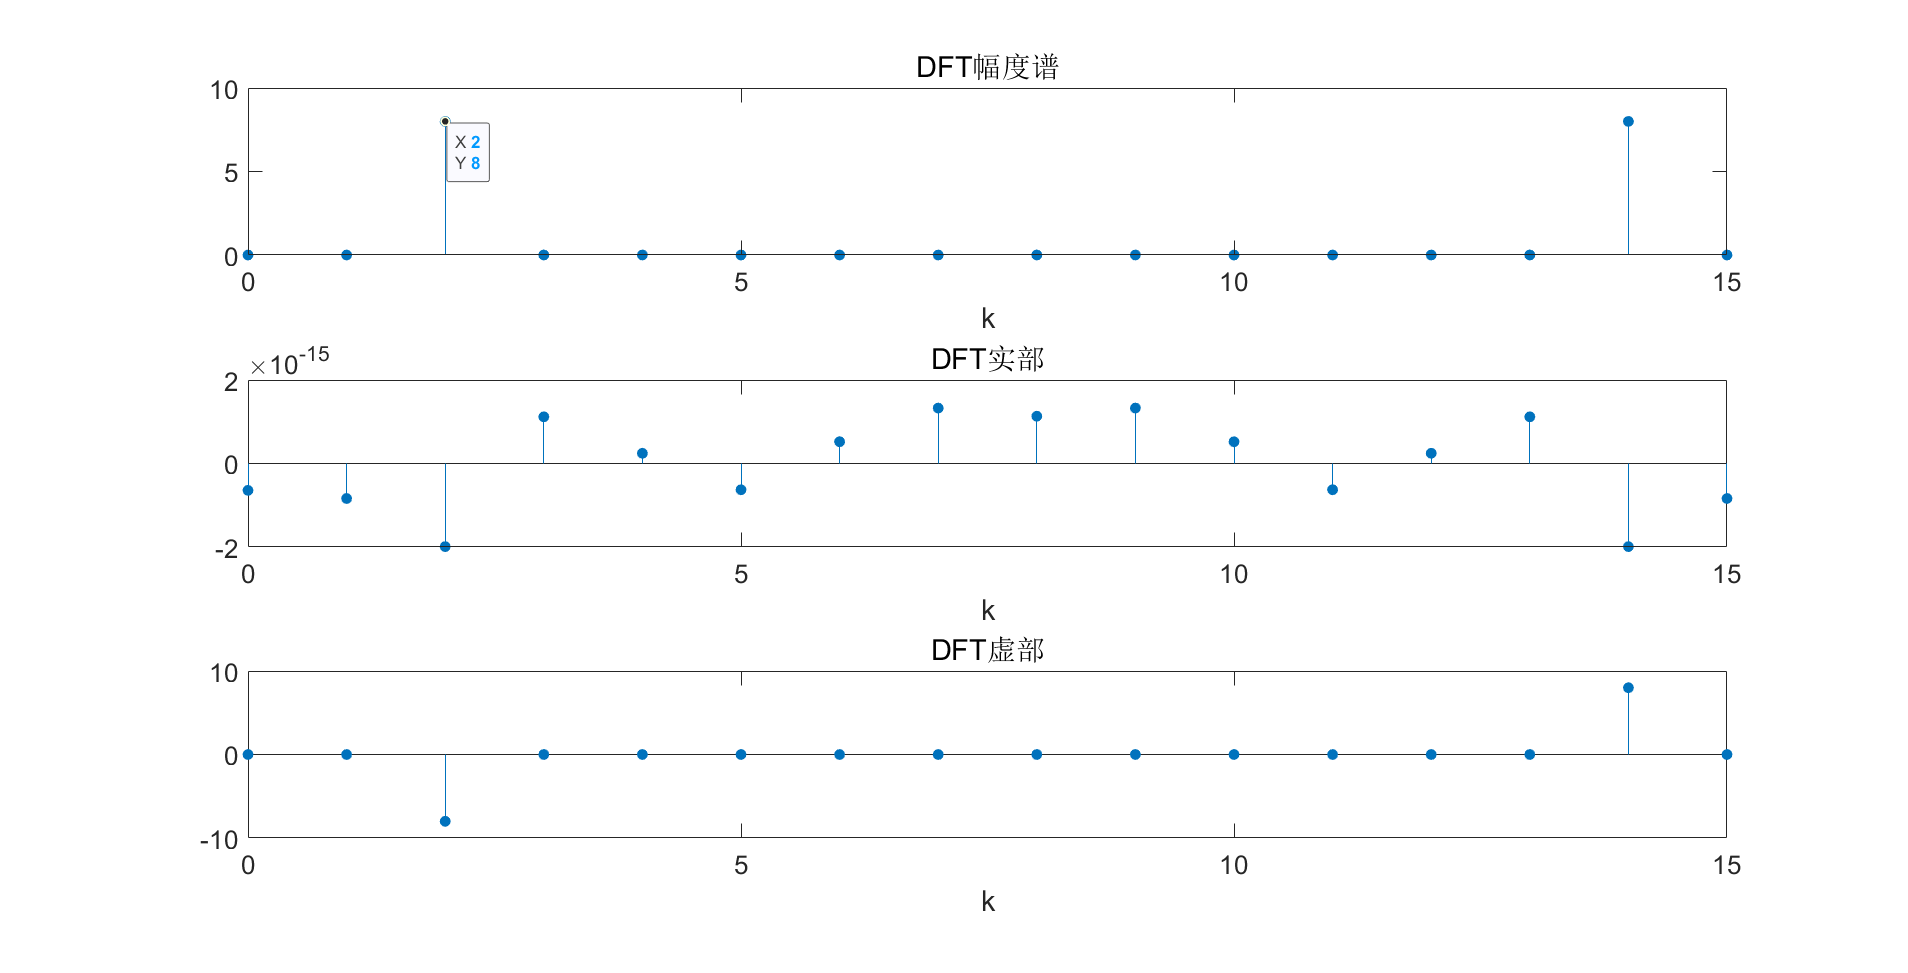
\includegraphics[width = \textwidth]{src/exp2_5_3.png}
                    \caption{第五组:f = 50Hz, T = 0.0025s, N = 16}
                \end{figure}
                结果分析
                \begin{table}[H]
                    \centering
                    \begin{tabular}{|c|c|c|c|c|c|c|}
                    \hline
                    组别    & 抽样间隔T     & 截断长度N  & 谱峰所在频率 & 谱峰的数值   & 是否混叠 & 是否频谱泄露 \\
                          & (秒)       & (抽样个数) & (U)    & (V)     &      &        \\ \hline
                    第一组参数 & 0.000625  & 32     & 1      & 16      & 否    & 否      \\ \hline
                    第二组参数 & 0.005     & 32     & 8      & 16      & 否    & 否      \\ \hline
                    第三组参数 & 0.0046875 & 32     & 7      & 10.2519 & 否    & 是      \\ \hline
                    第四组参数 & 0.004     & 32     & 6      & 11.965  & 否    & 是      \\ \hline
                    第五组参数 & 0.0025    & 16     & 2      & 8       & 否    & 否      \\ \hline
                    \end{tabular}
                \end{table}
        \subsection{现象解释}
        用基本理论、基本概念来解释各种现象。 

        \subsubsection{频域混叠}
        序列的频谱是被采样信号频谱的周期延拓,当采样频率不满足奈奎斯特定律时,也就是不能满足采样频率大于等于两倍的信号最高频率时,就会发生频谱混叠,使得采样后的信号序列频谱不能真实的反映原信号的频谱。

        \subsubsection{频谱泄露}

        采样后,对序列进行了截断,等同于于乘上了一个窗函数,在频谱上,相当于频域上与sinc函数进行卷积,因此采样后的信号总是存在高频分量,因此总是存在频域混叠的现象,也会存在频域泄露的现象。

        而如果DFT采集时间窗口内的信号的周期延拓与实际信号完全吻合,那么就不会出现泄漏现象。换句话说,对于周期信号,如果采集时间窗口内正好包含整数个信号周期,就能避免频谱泄漏。

        所以第一、二、五组不会出现频谱泄露的现象,第三、四组会出现频谱泄漏。
 
\end{document}